\documentclass[12pt]{book}
\usepackage{standalone}
\usepackage{apacite}
\usepackage{etoolbox}% for the \patchcmd
\makeatletter
% Patch after apacite got loaded!
\patchcmd{\nocite}{\@onlypreamble\document}{\documentclass\sa@documentclass}{}{}
\makeatother
\usepackage{graphicx}
\usepackage{subcaption}
\graphicspath{{C:/Users/huawei/Desktop/images/}} 
\usepackage{setspace}
\usepackage{booktabs}
\usepackage{tabularx}
\usepackage{xcolor}
\usepackage{amsmath}
\usepackage{pdflscape}
\usepackage[margin=3cm]{geometry}
\usepackage{multirow}
\usepackage{times}
\usepackage{fancyhdr}
\usepackage{color}
\usepackage{dcolumn}
\usepackage{siunitx}
\usepackage{array}
\usepackage{longtable}
\usepackage{pdftexcmds}


\raggedbottom

\renewcommand\baselinestretch{2}


\newcolumntype{d}[1]{D{.}{.}{#1}}
\def\sym#1{\ifmmode^{#1}\else\(^{#1}\)\fi}


\begin{document}
\chapter{Typical scoring of implicit measures}\label{chap:classicscore}
This chapter presents typical scoring procedures for the IAT and the SC-IAT data, as well as the development of new, open source tools for easily computing the scores for the IAT and the SC-IAT.

The typical scoring algorithms for both the IAT and the SC-IAT are illustrated and described. 
It is not unusual to find studies in which both the IAT and the SC-IAT have been administered together, and their performances, for example for predicting a behavioral outcome, have been compared. However, this comparison might be biased by many differences concerning both the administration and the scoring procedures of the two implicit measures. Therefore, new scoring algorithms have been introduced with the aim of reducing the noise due to external factors (i.e., the scoring procedure itself) in the comparison between implicit measures. 
The results of an empirical study in which the performance of typical and modified scoring algorithms have been compared in respect to the prediction of a behavioral outcome are reported.


The core computation of both the IAT and the SC-IAT scores is rather easy. Nonetheless, the many steps that have to be undertaken for preparing and cleaning the data make it an error-prone procedure, and compromise the reproducibility of the results. Since there is a lack of easy-to-use and open source tools for their computation, a Shiny app and an \verb*|R| package have been developed for the computation of the IAT and the SC-IAT \emph{D} scores. These tools are presented at the end of this chapter.

\section{The IAT \emph{D} score}\label{sec:iatD}
\citeA{Greenwald2003} introduced different variations of the \emph{D} score algorithm (Table \ref{tab:Doverview}). These variations result from the combination of the error correction strategies (``Error replacement'' in the Table) and the treatment for fast responses (``Lower tail treatment'' in the Table).
\begin{table}[th!]
	\centering \doublespacing
	\caption{\label{tab:Doverview} Overview of \emph{D} score algorithms. }
	\begin{tabular}{p{2.5cm}p{4.5cm}p{4.5cm}}
		\toprule
		Algorithm & Error replacement & Lower tail treatment\\\hline
		\emph{D}1 & Built-in correction & No \\
		\emph{D}2 & Built-in correction & Delete trials $<$ 400ms \\
		\emph{D}3 & Mean $+$ 2\emph{sd} & No\\
		\emph{D}4 & Mean $+$ 600ms & No \\
		\emph{D}5 & Mean $+$ 2\emph{sd} & Delete trials $<$ 400ms\\
		\emph{D}6 & Mean $+$ 600ms & Delete trials $<$ 400ms \\
		\bottomrule
		\multicolumn{3}{p{12cm}}{\onehalfspacing\emph{Note:} For all algorithms, trials with latency $>$ 10,000ms are discarded. For the algorithm in which error responses are replaced with the average response time plus a penalty, the average response time is computed on correct responses only.}
	\end{tabular}
\end{table}

Blocks B1, B2, and B5 in Table \ref{tab:iatstructure} are considered as pure practice blocks and are hence discarded from the computation. Only trials from Blocks B3, B4 (i.e., Mapping A) and B6, B7 (i.e., Mapping B ) are used for the computation.  

The error correction strategies based on built-in correction (\emph{D1} and \emph{D2}) refer to the IAT procedure including feedback, according to which  respondents have to correct their error responses. The response time considered for the computation of the \emph{D} score is the response time at the first (incorrect) response inflated by the time required to correct it. All other algorithms (from \emph{D1} to \emph{D6} in Table \ref{tab:Doverview}) use a \emph{post-hoc} error correction strategy, for which error responses are replaced by the average response time of the correct responses in the block in which the error occurred increased by a standard penalty (i.e., either 600ms or twice the standard deviation).
The other feature differentiating the \emph{D} score algorithms is the lower tail treatment, according to which fast trials (trials faster than $400$ms) are discarded or not.

Regardless of the specific features of each algorithm, the core procedure for computing the \emph{D} score is the same. Firstly, the \emph{D} scores of associative practice blocks (Eq. \ref{eq:practice}):
%
\begin{equation}\label{eq:practice}
D_{\text{practice}} = \frac{M_{\text{B6}} - M_{\text{B3}}}{\text{\emph{SD}}_{\text{B6, B3}}}, 
\end{equation}
%
and of associative test blocks (Eq. \ref{eq:test}) 
%
\begin{equation}\label{eq:test}
D_{\text{test}} = \frac{M_{\text{B6}} - M_{\text{B3}}}{\text{\emph{SD}}_{\text{B6, B3}}},
\end{equation}
are computed.
In both cases, the difference in the average response time between the two critical blocks is divided by the standard deviation computed on the pooled trials of both blocks. Once $D_{\text{practice}}$ and $D_{\text{test}}$ are obtained, it is possible to compute the actual \emph{D} score: 
%
\begin{equation}\label{eq:dscore}
\text{\emph{D} score} = \frac{D_{\text{practice}} + D_{\text{test}}}{2}.
\end{equation}

The block order in Equation \ref{eq:practice} and Equation \ref{eq:test} is arbitrary and can be reversed. The resulting \emph{D} has to be interpreted accordingly. 
In the Coke-Pepsi IAT in Chapter \ref{chap:intro}, Blocks B3 and B4 constituted the Coke-Good/Pepsi-Bad condition. 
Conversely, the Pepsi-Good/Coke-Bad condition was composed of Blocks B6 and B7.
If the \emph{D} score is computed following the order of the blocks in Equation \ref{eq:practice} (i.e., $M_{\text{B6}} - M_{\text{B3}}$) and in Equation \ref{eq:test} (i.e.,$M_{\text{B7}} - M_{\text{B4}}$), a positive score would indicate slower responses in Pepsi/Good-Coke/Bad condition than in Coke/Good-Pepsi/Bad one, probably indicating a preference for Coke over Pepsi. Vice versa, if the order of the Block in Equations \ref{eq:practice} and \ref{eq:test} is reversed (i.e., $M_{\text{B3}} - M_{\text{B6}}$ and $M_{\text{B4}} - M_{\text{B7}}$, respectively), a positive score would indicate slower responses in the Coke/Good-Pepsi/Bad condition than in the Pepsi/Good-Coke/Bad condition, indicating a possible preference for Pepsi over Coke.


\section{The SC-IAT \emph{D} score}\label{sec:sciatD}

Since blocks B1 and B3 (Table \ref{tab:sciatstructure}) are considered as pure practice blocks, they are discarded from the computation of the SC-IAT \emph{D} score. If a rtw was included in the administration procedure, all responses exceeding it are considered as non-responses and are discarded from the computation. All responses with a latency faster than 350ms are discarded, and error responses are replaced with the average response time of the block in which the error occurred inflated by a standard penalty of 400ms. 

After cleaning and preparing the data, the SC-IAT \emph{D} score is simply computed as the difference in the average response time of the two critical blocks (i.e., $M_{\text{B4}} - M_{\text{B2}}$) divided by the standard deviation computed of the correct trials of both blocks. As for the IAT, the order of the critical blocks is arbitrary and the interpretation of the \emph{D} score changes accordingly. 

In the Coke SC-IAT example illustrated in Chapter \ref{chap:intro}, Block B2 was the Coke-Good condition, while Block B4 was the Coke-Bad condition.
Following this structure, if the \emph{D} score is computed by taking the difference between Blocks B4 and B2, a positive score would indicate slower responses in the Bad/Coke condition than in the Good/Coke one, standing for a positive evaluation of Coke. Vice versa, if the score is computed in the opposite direction (i.e., $M_{\text{B2}} - M_{\text{B4}}$), a positive score would indicate slower responses in the Good/Coke condition than in the Bad/Coke condition, indicating a plausible negative evaluation of Coke. 


\section[A fairer comparison]{A fairer comparison between the IAT and the SC-IAT}

In Study 1, \citeA{karpinski2006} directly investigated and compared the predictive ability of a Coke-Pepsi IAT, that of a Coke SC-IAT, and that of a Pepsi SC-IAT. 
the behavioral outcome was the choice between a can of Coke and a can of Pepsi.
As their results suggested, measures obtained from both the Coke-Pepsi IAT and the Pepsi SC-IAT played  a role in predicting the soda choice, while the measure obtained from the Coke SC-IAT did not contribute to the choice prediction. 
%\citeA[Study 1]{karpinski2006} provided a direct comparison between the IAT and the SC-IAT. These authors investigated the capacity of a Coke-Pepsi IAT, a Coke SC-IAT and a Pepsi SC-IAT of predicting the soda choice between Coke and Pepsi. Results showed that both the Coke-Pepsi IAT and the Pepsi SC-IAT allowed for predicting the soda choice, while the Coke SC-IAT was unrelated to the choice. 
Drawing on these results, authors speculated that the soda choice is more guided by a positive evaluation of Pepsi than by a negative evaluation of Coke. Nonetheless, the direct comparison between the predictive ability of the two implicit measures has been poorly investigated. 
Despite the study by \citeA{karpinski2006} provided interesting information on the functioning of implicit processes and the comparison between implicit measures, it also had some shortcomings that might have undermined the validity of their results. 
The aim of the study reported in this section was to to provide a fairer comparison of the predictive ability of the IAT and the SC-IAT in respect to a behavioral choice by presenting new  scoring algorithms for the two implicit measures. This study is published in \citeA{fairer}.

Among the shortcomings in \citeA{karpinski2006}, the sample size was rather small, and results should hence be interpreted with caution. Moreover, the comparison between the predictive ability of the implicit measures might have been affected by issues concerning their administration and scoring procedures. 
The IAT and the SC-IAT differed in the number of trials, the number of blocks, and the number of exemplars representing each category. 
The SC-IAT employed more trials and more stimuli than the IAT, for both the evaluative dimensions (twenty-one exemplars for each SC-IAT evaluative dimension versus five exemplars for each IAT evaluative dimension) and the object categories (seven exemplars for each SC-IAT target object category and five exemplars for each IAT target object category). 
Furthermore, the administration of the SC-IAT included a rtw, while that of the IAT did not have such a constraint on the responses. The presence of a rtw makes the task more difficult and produces a sense of urgency that is otherwise missing \cite{karpinski2006}. 
Additionally, in the SC-IAT respondents were given feedback for each correct and incorrect response, while the IAT administration procedure did not include any feedback. 
The labels used for representing the positive and negative evaluative dimensions changed across implicit measures (\emph{Pleasant} vs \emph{Unpleasant} for the IAT and \emph{Good} vs \emph{Bad} for the SC-IAT), as well as the response keys used for sorting the stimuli.  The IAT \emph{D} score was computed according to the \emph{D} score procedure in \citeA{Greenwald2003}, despite \citeA{karpinski2006} failed to report the exact algorithm they employed. The SC-IAT \emph{D} score presented in Section \ref{sec:sciatD} was used for computing the SC-IAT \emph{D} score.

%To the best of our knowledge, only \citeA{karpinski2006} provided a systematic comparison between the predictive ability of the two implicit measures. However, their study presented some drawbacks that might have undermined the validity of their results. Firstly, the sample size was rather small, and results should hence be interpreted with caution. Moreover, the comparison between the predictive ability of the two implicit measures might have been affect by issues concerning bothe their administration and scoring procedures. The IAT and the SC-IAT differed in both the number of trials and the number of stimuli used for representing each category. The SC-IAT employed more stimuli than the IAT, for both the evaluative dimensions (twenty-one stimuli for each SC-IAT evaluative dimension versus five stimuli for each IAT evaluative dimension), and the object stimuli (seven stimuli for each SC-IAT target object category and five stimuli for each IAT target object category). Furthermore, the administration of the SC-IAT included a response time window (RTW), for which after 1,500ms the stimulus on the screen disappeared. Conversely, the IAT did not have such a constraint on the responses. Beyond making the task more difficult, the presence of a RTW induce a sense of urgency of giving the response which is missing when the RTW is not included \cite{karpinski2006}. According to SC-IAT administration procedure presented in Section \ref{sec:sciat}, respondents were given feedback for each correct and incorrect response,while this was not done in the IAT case. The procedures differed also on the labels used for representing the positive and negative attribute categories (\emph{Pleasant} and \emph{Unpleasant} for the IAT and \emph{Good} and \emph{Bad} for the SC-IAT), and on the response keys used for sorting the stimuli.  The IAT \emph{D} scores were computed according to the \emph{D} score procedure in \citeA{Greenwald2003}, despite \citeA{karpinski2006} fails to report the exact algorithm they have employed. The SC-IAT \emph{D} score presented in Section \ref{sec:sciatD} was used for computing the SC-IAT \emph{D} score.

Given the differences between administration and scoring, the comparison between the ability of the IAT and that of the SC-IAT to predict a behavioral outcome might have been unfair. To the best of our knowledge, there is neither a scoring procedure employing the same criteria for both the IAT and the SC-IAT, nor an attempt to align the two implicit procedures to allow for a fairer comparison between their predictive ability. 
It would be interesting to compare the predictive ability of the two implicit measures by using the same scoring procedure on their data and by keeping the administration as similar as possible, while acknowledging their key features (e.g., block types and usual length of the blocks). 
If by using the same scoring procedure and by reducing the administration-related differences there are still differences in the predictive ability of the two measures, these differences can be reasonably attributed to the implicit procedure itself.

To obtain a fairer comparison between the two implicit measures, both administration (e.g., stimuli, rtw, feedback) and scoring of the two procedures have been aligned.

\subsection{Method}\label{sub:fairerMethod}

To test the predictive ability of the new scoring procedures, one Chocolate IAT, one Dark chocolate SC-IAT, and one Milk chocolate SC-IAT were developed. 
The decision to use chocolate as the object category was driven by different reasons. Firstly, chocolate preference should not be sensitive to social desirability, and hence respondents would have no concerns in explicitly reporting their actual chocolate preference. Moreover, it offers the chance to ask for a behavioral choice disguised as a reward for the participation.

Inquisit 3.0 \cite{inquisit3} was used for administering the implicit measures (i.e., the IAT and the two SC-IATs) and the demographic questionnaire.


\paragraph{Participants.}

Participants were recruited at the University of Padova. One-hundred and sixty-one people (F $= 63.55$\%, Age $= 23.95 \pm 2.83$) volunteered to take part in the study, with no compensation. Participants were informed about the confidentiality of the data, and they were given the possibility to withdraw from the experiment at any time they wished. They were asked for their consent to take part in the study. Majority of the participants were students ($94.08$\%), including both undergraduates, master, and PhD students. Only two participants reported to have a PhD title, while the majority reported to have a bachelor’s degree (43.42\%), immediately followed by those who reported having a high school diploma (32.24\%) and a master’s degree (23.03\%). 

\paragraph{Materials and Procedure.}

Chocolate stimuli were composed by seven images of chocolate that were modified to represent either Dark or Milk chocolate. Seven images for each type of chocolate were used. Three independent judges evaluated the stimuli regarding their properties, specifically whether they were clearly identifiable as dark or milk chocolate images. The three judges agreed on the representativeness of the stimulus in respect to the category it was supposed to to belong. All chocolate images were presented on a white background. 
%The stimuli and the Inquisit script for running the experiment can be retrieved in an online repository (\url{https://osf.io/cnq4u/}). 

In the Chocolate IAT, both Dark and Milk chocolate images were used. In the two SC-IATs, only either dark (Dark SC-IAT) or milk (Milk SC-IAT) chocolate images were used. Object categories were labeled \emph{Dark} or \emph{Milk}. Evaluative attributes categories were composed of 13 stimuli each. The evaluative categories were labeled as \emph{Positive} (i.e., ``good'', ``laughter'', ``pleasure'', ``glory'', ``peace'', ``happiness'', ``joy'', ``love'', ``wonderful'', ``beautiful'', ``excellent'', ``heaven'', ``marvelous'') or \emph{Negative} (i.e., ``evil'', ``bad'', ``horrible'', ``terrible'', ``annoying'', ``pain'', ``failure'', ``hate'', ``nasty'', ``disaster'', ``agony'', ``ugly'', ``disgust'').  
Response key ``E'' was used for sorting the stimuli belonging to the categories represented on the left-side of the screen. Response key ``I'' was used for sorting the stimuli belonging to the categories represented on the right side of the screen.  
The SC-IAT practice Blocks B1 and B3 were composed of 20 trials, as for the practice blocks of the IAT. 
Neither the IAT nor the SC-IATs included any feedback or rtw. Respondents were asked to be as fast and as accurate as they could in performing the tasks. 

Respondents were explicitly asked to report their evaluation for Dark and Milk chocolate on two distinct items (``How much do you like Dark chocolate?'' and ``How much do you like Milk chocolate?'') rated from ``0 – Not at all'' to ``5 – Very much''.The order of presentation of the implicit measures was counterbalanced across participants, while the demographic questionnaire and the choice were kept constant at the end of the experiment.

As a reward for their participation, respondents were offered with either a free Dark chocolate bar or a Milk chocolate one. The experimenter registered respondents' choices after they left the laboratory.

\emph{Chocolate IAT:} The critical blocks were composed of 60 trials each (20 practice and 40 test), defining the Dark-Good/Milk-Bad condition (DGMB), and the Milk-Good/Dark-Bad condition (MGDB). 

\emph{Dark SC-IAT:} The critical blocks were composed of 72 trials each, defining the Dark-Good/Bad (DG) and the Good/Dark-Bad (DB) conditions.

\emph{Milk SC-IAT:} As for the Dark chocolate SC-IAT, the critical blocks were composed of 72 trials each, defining the Milk-Good/Bad (MG) and the Good/Milk-Bad (MB) conditions.

\subsection{Data analysis}
\subsubsection{Data cleaning and \emph{D} score}

All the IAT \emph{D} score algorithms not including a built-in correction (algorithms \emph{D}3, \emph{D}4, \emph{D}5 and \emph{D}6 in Table~\ref{tab:Doverview}) were computed. The procedure described in Section \ref{sec:sciatD} was followed for computing the SC-IAT \emph{D} score.

The scoring algorithms that have been introduced in this study result from different combinations of two main characteristics. One characteristic is the trials on which the standard deviation for the replacement of error responses was computed (i.e., only correct trials or all trials). The other characteristic is the quantity used for standardizing the difference in the response times between the associative conditions (i.e., Cohen's pooled standard deviation or pooled trials standard deviation). 
Cohen's pooled standard deviation for two groups of size $n_1$ and $n_2$ is as follow: 

\begin{equation}
	\text{\emph{SD}}_{\text{\emph{pooled}}} = \sqrt\frac{(n_1-1)SD_1 + (n_2 -1)SD_2}{n_1 + n_2 -2}
\end{equation}

The resulting eight combinations (identified by letter ``\emph{m}'', \emph{modified}) are illustrated in Table~\ref{tab:modified}. 

\begin{table}[h!]
	\centering \doublespacing 
	\caption{\label{tab:modified} Overview of modified algorithms for computing the IAT and the SC-IAT scores.}
	\begin{tabular}{l p{1cm} p{1cm}p{1cm} p{1cm}p{1cm} p{1cm}p{1cm} p{1cm}}
		\toprule
		Feature & \emph{m}1 & \emph{m}2  & \emph{m}3 & \emph{m}4 & \emph{m}5 & \emph{m}6 & \emph{m}7 & \emph{m}8 \\
		\midrule
		Lower tail treatment & \multicolumn{8}{c}{$<$ 350ms}\\
		Upper tail treatment & \multicolumn{8}{c}{$>$ 10,000ms}\\
		Error treatment & \multicolumn{4}{c}{Mean (Correct) $+$ 2 \emph{sd} (Correct)}  & \multicolumn{4}{c}{Mean (Correct) $+$ 2 \emph{sd}}\\
		Denominator & \multicolumn{2}{c}{Pooled trials} & \multicolumn{2}{c}{Cohen} & \multicolumn{2}{c}{Pooled trials} & \multicolumn{2}{c}{Cohen}\\  
		Denominator trials & Correct & All  & Correct & All & Correct & All & Correct & All \\
		\bottomrule
	\end{tabular}
\end{table}

While the typical procedure for the SC-IAT includes a default lower tail treatment, the lower tail treatment for the IAT depends on the specific \emph{D} score algorithm (see Table~\ref{tab:Doverview}). To have a comparable score, a common lower tail treatment for both procedures was set (i.e., responses with a latency less than 350ms were discarded). 
Since it is not uncommon to find SC-IATs with no rtw, a common upper tail treatment for response times was proposed for both implicit measures (i.e., responses over 10,000ms were discarded). Concerning the SC-IAT upper tail treatment, it might be argued that the deletion of the responses higher than 1,500ms (i.e., the rtw cut-off) would be a more appropriate threshold for slow responses. Nonetheless, the presence of the rtw itself produce an urge to respond that is missing when the rtw is not included in the administration procedure \cite{karpinski2006}. 

Since the SC-IAT is known to be an easier task than the IAT \cite{karpinski2006}, the latency of the responses in the SC-IAT tend to be faster than the latency of the responses in the IAT. Therefore, assuming 600ms as a reasonable time for correcting the error response might be a too strong assumption for the SC-IAT data. Conversely, the penalty used in the SC-IAT (400ms) might be not enough for acknowledging the response time needed for correcting the error response in the IAT. For this reason, the error responses are replaced by the average response times in the block in which the error occurred inflated by two times the standard deviation of the block.  

The pooled trials standard deviation and the Cohen’s pooled standard deviation were computed either considering only correct responses or all trials. In the former case, the variability due to incorrect responses is not accounted for, while it is addressed in the latter case.
Finally, the IAT modified procedures were computed as the difference between the two associative conditions, instead of as the mean of the standardized average response time differences between the practice and test blocks.

The IAT scores (typical and modified) were computed so that positive scores indicated faster responses in associating Milk chocolate with positive attributes and Dark chocolate with negative attributes, and hence an implicit preference for Milk chocolate over Dark chocolate. Conversely, negative scores indicated faster responses in associating Dark chocolate with positive attributes and Milk chocolate with negative attributes, indicating an implicit preference for Dark chocolate over Milk chocolate. 

For the SC-IATs, both typical and modified procedures were computed so that positive scores indicated faster responses in associating the target chocolate with positive attributes than with negative attributes, hence indicating an implicit positive evaluation of the target chocolate. Conversely, negative scores indicated faster responses when the target chocolate was associated with negative attributes, and an implicit negative evaluation of the target chocolate.

\subsubsection{Consistency between modified and typical scores, and relationship with explicit measures}

Pearson's correlations between explicit chocolate evaluations, typical and modified scoring were computed. 
Moreover, Pearson's correlations were computed between the typical and modified scores to check for their consistency. 


\subsubsection{Prediction of the behavioral outcome}\label{subsub:predchoice}

The typical and the modified scores are regressed on the  chocolate choice, coded as 0 for the Dark chocolate choice (DCC) and 1 for the Milk chocolate choice (MCC).
Each score is regressed on the choice in a separate logistic regression. 
Since the choice is presented as a dichotomous task in which Dark chocolate is contrasted with Milk chocolate, it is plausible that the relative preference for one chocolate over the other plays a role in determining the actual choice. 
The score of each SC-IAT conveys a unique information on the absolute positive or negative evaluation of one type of chocolate. As such, each of them lacks a part of information that might be crucial in predicting the choice. 
The use of the linear combination of both SC-IATs scores or a combined score might solve this issue. However, since the SC-IATs scores are obtained from two different experiments, their combination, either linear or in a comprehensive score, might be considered a stretch.
Grounding on these considerations, both the single Dark SC-IAT score and the single Milk SC-IAT score, as well as their linear combinations, were used for predicting the choice.

Nagelkerke’s \emph{R}$^2$ \cite{nagel} and model accuracy of prediction \cite{faraway2006} are used as criteria for investigating the scores best accounting for the behavioral choice. 
Specifically, model general accuracy (i.e., ratio between the number of chocolate choices correctly identified by the model and the total number of choices), DCC accuracy (i.e., ratio between the number of DCCs correctly identified by the model and the total number of observed DCCs), and MCC accuracy (i.e., ratio between the number of MCCs correctly identified by the model and the total number of observed MCCs) are computed.

\subsection{Results}\label{fairer:results}

Data from nine participants were discarded. Eight of them explicitly reported not understanding the tasks they were asked to perform in either the IAT or one of the SC-IATs, while one of them registered too many fast responses, specifically on the Dark chocolate SC-IAT (more than 30\% of responses with a latency lower than 350ms). 
The final sample was composed of 152 participants (F $= 63.82$\%, Age $= 24.03 \pm 2.8$2). Milk chocolate was chosen by the $48.03$\% of the participants. 

The median for the explicit evaluation of Dark chocolate was 3 ($Q_{1}$ = 2, $Q_{3}$ = 5). The median for the explicit evaluation of Milk chocolate was 4 ($Q_1$ = 3, $Q_3$ = 4). No trials exceeding the threshold of 10,000ms were found in the SC-IATs. Three trials exceeding the 10,000ms threshold were found in the IAT, and they were eliminated. 
The lowest percentages of trials faster than both $400$ms ($1.39$\%) and $350$ms ($0.19$ \%) were found in the IAT. The two SC-IATs showed similar percentages of trials faster that $350$ms ($1.00$\% and $0.90$\% in Milk SC-IAT and Dark SC-IAT, respectively), as well as of trials faster than $400$ms ($4.40$\% and $4.32$\% in Dark SC-IAT and in Milk SC-IAT, respectively).
All implicit measures had the same overall percentage of correct responses ($95$\%).

In the IAT, the overall average response time was $862.03$ms (\emph{sd} $= 496.50$, \emph{skewness} $= 3.45$, \emph{kurtosis} $= 22.01$). The average response time in the DGMB condition was $976.44$ms (\emph{sd} $= 555.19$, \emph{skewness} $= 2.88$, \emph{kurtosis} $= 14.01$) and that in the MGDB condition was $747.62$ms (\emph{sd} $= 398.30$, \emph{skewness} $= 4.76$, \emph{kurtosis} $= 48.62$). 

The overall average response time in the Dark SC-IAT was $679.45$ms (\emph{sd} $= 328.72$, \emph{skewness} $= 4.10$, \emph{kurtosis} $= 27.94$). The average response time in the DB condition was $673.71$ms (\emph{sd} $= 322.87$, \emph{skewness} $= 3.90$, \emph{kurtosis} $= 24.46$) and that in the DG condition was $685.19$ms (\emph{sd} $= 334.39$, \emph{skewness} $= 4.27$, \emph{kurtosis} $= 30.86$). 

The overall average response time in the Milk SC-IAT was $675.90$ms (\emph{sd} $= 322.31$, \emph{skewness} $= 4.48$, \emph{kurtosis} $= 38.19$). The average response time in the MB condition was $695.72$ms (\emph{sd} $= 344.84$, \emph{skewness} $= 4.10$, \emph{kurtosis} $= 28.32$) and that in the MG condition was $656.08$ms (\emph{sd} $= 296.78$, \emph{skewness} $= 4.98$, \emph{kurtosis} $= 54.05$). 

\paragraph{Relationship with explicit measures.}

Descriptive statistics for the typical scoring of all implicit measures, along with their correlation with explicit measures, are reported in Table~\ref{tab:Faircorrclassic}. 

\begin{landscape}
	\begin{table}[h!]
		\caption{\label{tab:Faircorrclassic} Descriptive statistics of the scores and correlations ($r$) with explicit chocolate evaluations.}
		\centering \onehalfspacing
		\resizebox{\linewidth}{!}{
			%\small
			\begin{tabular}{ll d{2.7} d{2.2} d{2.2} d{1.5} d{1.5} l d{2.7} d{2.2}d{2.2}d{1.5}d{1.5}}
				\toprule
				& Modified & \multicolumn{1}{l}{\emph{M (sd)}}& \multicolumn{1}{l}{\emph{Min}} & \multicolumn{1}{l}{\emph{Max}} &\multicolumn{1}{l}{\emph{r}\textsubscript{Milk}} & \multicolumn{1}{l}{\emph{r}\textsubscript{Dark}}  & Typical &\multicolumn{1}{l}{\emph{M (sd)}} & \multicolumn{1}{l}{\emph{Min}} & \multicolumn{1}{l}{\emph{Max}} & \multicolumn{1}{l}{\emph{r}\textsubscript{Milk}} & \multicolumn{1}{l}{\emph{r}\textsubscript{Dark}} \\ \midrule
				IAT  &  \emph{m1}   & 0.64\,(0.62) & -1.91 & 1.72 & 0.40\sym{***}&-0.36\sym{***} &  \emph{D3}   & 0.41\,(0.41)  & -1.29 & 1.25 & 0.42\sym{***} & -0.38\sym{***}\\
				&  \emph{m2}   & 0.64\, (0.60) & -1.86 & 1.69 & 0.40\sym{***}&-0.37\sym{***} &  \emph{D4}   & 0.39\, (0.39)  & -1.26 & 1.27 & 0.41\sym{***} & -0.38\sym{***}\\
				&  \emph{m3}   & 0.73\, (0.73) & -2.25 & 2.84 & 0.39\sym{***}&-0.34\sym{***} &  \emph{D5}   & 0.40\, (0.41)  & -1.29 & 1.29 & 0.42\sym{***} & -0.37\sym{***}\\
				&  \emph{m4}   & 0.72\, (0.70) & -2.12 & 2.59 & 0.39\sym{***}&-0.35\sym{***} &  \emph{D6}   & 0.39\, (0.39) & -1.26 & 1.32 & 0.41\sym{***} & -0.37\sym{***}\\
				& \emph{m5}   & 0.64\, (0.63) & -2.29 & 1.72 & 0.40\sym{***}&-0.35\sym{***} &                  &  &              &    &  & \\
				& \emph{m6}   & 0.64\, (0.60) & -1.85 & 1.69 & 0.40\sym{***}&-0.36\sym{***} &                  &  &              &    &  & \\
				& \emph{m7}   & 0.72\, (0.75) & -2.34 & 2.85 & 0.39\sym{***}&-0.34\sym{***} &                  &  &              &    &  & \\
				& \emph{m8}   & 0.72\, (0.71) & -2.11 & 2.60 & 0.39\sym{***}&-0.35\sym{***} &                  &  &              &    &  & \\
				Dark SC-IAT  &   \emph{m1}   & -0.06\, (0.35) & -0.98 & 1.07 & -0.22\sym{**}&0.18\sym{*} &  \emph{D-Dark}    & -0.05\,(0.31)  & -0.74 & 0.78 & -0.19\sym{*} & 0.17\sym{*}\\
				& \emph{m2}   & -0.06\, (0.34) & -1.03 & 0.94 & -0.23\sym{**}&0.17\sym{*} &     &     &     &     &     &  \\
				& \emph{m3}   & -0.06\, (0.36) & -1.01 & 1.07 & -0.22\sym{**}&0.17\sym{*} &     &     &     &     &     &  \\
				&  \emph{m4}   & -0.06\, (0.35) & -1.05 & 0.94 & -0.22\sym{**}&0.17\sym{*} &     &     &     &     &     &  \\
				&  \emph{m5}   & -0.06\, (0.36) & -1.00 & 1.13 & -0.20\sym{*}&0.16\sym{*} &     &     &     &     &     &  \\
				&  \emph{m6}   & -0.06\, (0.35) & -0.95 & 0.99 & -0.20\sym{*}&0.16 &     &     &     &     &     &  \\
				&  \emph{m7}   & -0.06\, (0.36) & -1.04 & 1.13 & -0.19\sym{*}&0.16 &     &     &     &     &     &  \\
				&  \emph{m8}   & -0.06\, (0.35) & -0.97 & 1.00 & -0.20\sym{*}&0.16 &     &     &     &     &     &  \\
			Milk SC-IAT  &   \emph{m1}   & 0.16\,(0.39) & -1.92 & 1.22 & 0.17\sym{*}&0.04 &  \emph{D-Milk}    & 0.15\, (0.33)  & -0.93 & 1.21 & 0.13 & 0.06\\
				&   \emph{m2}   & 0.16\, (0.39) & -1.93 & 1.13 & 0.17\sym{*}&0.04 &     &     &     &     &     &  \\
				&  \emph{m3}   & 0.16\, (0.41) & -1.92 & 1.5 & 0.17\sym{*}&0.04 &     &     &     &     &     &  \\
				&   \emph{m4}   & 0.16\, (0.40) & -1.94 & 1.38 & 0.17\sym{*}&0.04 &     &     &     &     &     &  \\
				&  \emph{m5}   & 0.16\, (0.38) & -1.39 & 1.23 & 0.15&0.05 &     &     &     &     &     &  \\
				&  \emph{m6}   & 0.16\, (0.37) & -1.40 & 1.14 & 0.15&0.05 &     &     &     &     &     &  \\
				&  \emph{m7}   & 0.17\, (0.39) & -1.39 & 1.51 & 0.16\sym{*}&0.05 &     &     &     &     &     &  \\
				&   \emph{m8}   & 0.16\, (0.39) & -1.40 & 1.39 & 0.16\sym{*}&0.05 &     &     &     &     &     &  \\
				\bottomrule
				\multicolumn{13}{p{18cm}}{\emph{Note:} $\sym{***}$ $p < .001$, $\sym{**}$ $p < .01$, $\sym{*}$ $p < .05$. \emph{m}: Modified scoring algorithms; \emph{D}: Typical scoring algorithms}
			\end{tabular}
		}
	\end{table}
\end{landscape}

Regardless of the scoring algorithm, the SC-IAT scores tended to have smaller effect sizes than the IAT scores.
The IAT modified scores showed higher effect sizes than the IAT typical scores. The modified and typical SC-IAT scores were more consistent between each other. 

The explicit Dark chocolate evaluation negatively and moderately correlated with the explicit Milk chocolate evaluation ($r = -.39$, $p < .001$). The IAT and the Dark SC-IAT typical scores significantly correlated with both explicit chocolate evaluations. 
The Milk SC-IAT typical score correlated with neither the Dark nor the Milk explicit evaluation. The IAT modified scores significantly and moderately correlated with the explicit evaluations of both Dark and Milk chocolate.
The modified scores of both SC-IATs significantly correlated with the explicit evaluation of Milk chocolate. Only the first four modified scores of the Dark SC-IAT significantly correlated with the explicit evaluation of Dark chocolate. 
The correlation between the explicit evaluation of Dark chocolate and the scores of the Milk SC-IAT (both typical and modified) was near zero. 

\paragraph{Consistency between typical scores, modified scores, and explicit measures.}

The correlation coefficients between the typical IAT \emph{D} scores ranged between $.99$ and $1.00$ (all $p$s $< .001$). The correlations between the typical IAT scores and the Dark SC-IAT typical score were all $-.21$ (all $p$s $<.01$). 
No correlations were found between the typical IAT \emph{D} scores and the typical Milk SC-IAT score (correlations ranged between $-.04$ and $-.03$, all $p$s $>.05$). The typical \emph{D-Dark} and \emph{D-Milk} positively correlated between each other ($r = .15$, $p > .05$), but the correlation was not significant. 
The correlations between IAT modified scores ranged between $.97$ and $.99$ (all $p$s $< .001$). 
Their correlations with modified the \emph{D-Dark} ranged between $-.31$ and $-.28$ (all $p$s $<.001$). 
The modified \emph{D-Milk} and the modified IAT \emph{D} scores did not correlate with each other (correlation coefficients ranged between $-.01$ and $.01$, all $p$s $> .050$). 
The correlations between modified \emph{D-Dark} ranged between $.98$ and $1.00$ (all $p$s $<.001$). The correlations between modified \emph{D-Milk} ranged between $.99$ and $1.00$ (all $p$s $<.001$). The correlations between modified \emph{D-Milk} and \emph{D-Dark} showed the same direction as the correlation between typical SC-IAT scores, ranging between $.15$ and $.20$. 
Interestingly, the correlation between all modified \emph{D-Milk} and modified \emph{D-Dark} from 5 to 8 (i.e., the scores in which  error responses were replaced by the mean added with twice the standard deviation computed on all trials) showed slightly stronger and significant correlations, ranging from $.18$ and $.20$ (all $p$s $<.010$). 

\paragraph{Behavioral outcome.}

 Results of the logistic regressions for predicting the chocolate choice are reported in Table \ref{tab:Fairsingchoice}.

\begin{landscape}
	\begin{table}
	\caption{\label{tab:Fairsingchoice} Choice prediction results, single predictors..}
	\centering \onehalfspacing
	\resizebox{\linewidth}{!}{
		\begin{tabular}{p{1.5cm} D{,}{.}{1} D{,}{.}{1} D{,}{.}{1}  D{,}{.}{1}  D{,}{.}{1}  p{1.5cm}  D{,}{.}{1}  D{,}{.}{1}  D{,}{.}{1}  D{,}{.}{1}  D{,}{.}{1} }
		\toprule
		\multicolumn{1}{c}{} & \multicolumn{1}{l}{$B \, (se)$} & \multicolumn{1}{l}{\emph{Pseudo R}$^2$} & General & DCC & MCC & & \multicolumn{1}{c}{$B \, (se)$}  & \multicolumn{1}{c}{\emph{Pseudo R}$^2$} & General & DCC & MCC \\
		\midrule
IAT \emph{m1}  	 & 	  1.35 \sym{***} \, (0.34)  	  & 	0.16	  & 	0.64	  & 	0.65	  & 	0.63	 & 	\emph{D3}  	 & 	  2.23 \sym{***} \, (0.54)  	  & 	0.18	  & 	0.64	  & 	0.63	  & 	0.66	  \\
IAT \emph{m2}  	 & 	  1.38 \sym{***} \, (0.35)   	  & 	0.16	  & 	0.62	  & 	0.62	  & 	0.63	 & 	\emph{D4}  	 & 	  2.26\sym{***} \,(0.55)   	  & 	0.18	  & 	0.64	  & 	0.66	  & 	0.63	  \\
IAT \emph{m3}  	 & 	  1.07 \sym{***} \, (0.28)  	  & 	0.15	  & 	0.63	  & 	0.65	  & 	0.62	 & 	\emph{D5}  	 & 	  2.18\sym{***} \, (0.53)  	  & 	0.18	  & 	0.63	  & 	0.63	  & 	0.63	  \\
IAT \emph{m4}  	 & 	  1.12 \sym{***} \, (0.29)   	  & 	0.15	  & 	0.64	  & 	0.66	  & 	0.63	 & 	\emph{D6}  	 & 	  2.22\sym{***} \, (0.55)   	  & 	0.17	  & 	0.64	  & 	0.65	  & 	0.63	  \\
IAT \emph{m5}  	 & 	  1.35 \sym{***} \, (0.34)   	  & 	0.16	  & 	0.64	  & 	0.65	  & 	0.63	 & 		 & 		  & 		  & 		  & 		  & 		  \\
IAT \emph{m6}  	 & 	  1.38 \sym{***} \, (0.35)  	  & 	0.16	  & 	0.64	  & 	0.63	  & 	0.64	 & 		 & 		  & 		  & 		  & 		  & 		  \\
IAT \emph{m7}  	 & 	  1.07 \, (0.28)   	  & 	0.15	  & 	0.63	  & 	0.65	  & 	0.62	 & 		 & 		  & 		  & 		  & 		  & 		  \\
IAT \emph{m8}  	 & 	  1.12\, (0.29)  	  & 	0.15	  & 	0.64	  & 	0.66	  & 	0.63	 & 		 & 		  & 		  & 		  & 		  & 		  \\
Dark \emph{m1}  	 & 	  -0.73\, (0.48)   	  & 	0.02	  & 	0.53	  & 	0.62	  & 	0.44	 & 	\emph{D-Dark}   	 & 	  -0.70 \sym{***} \, (0.54)   	  & 	0.01	  & 	0.53	  & 	0.65	  & 	0.41	  \\
Dark \emph{m2}  	 & 	  -0.72\, (0.49)   	  & 	0.02	  & 	0.53	  & 	0.62	  & 	0.42	 & 		 & 		  & 		  & 		  & 		  & 		  \\
Dark \emph{m3}  	 & 	  -0.70\, (0.47)   	  & 	0.02	  & 	0.53	  & 	0.62	  & 	0.44	 & 		 & 		  & 		  & 		  & 		  & 		  \\
Dark \emph{m4}  	 & 	  -0.69\, (0.48)   	  & 	0.02	  & 	0.52	  & 	0.62	  & 	0.41	 & 		 & 		  & 		  & 		  & 		  & 		  \\
Dark \emph{m5}  	 & 	  -0.62\, (0.47)   	  & 	0.02	  & 	0.52	  & 	0.63	  & 	0.4	 & 		 & 		  & 		  & 		  & 		  & 		  \\
Dark \emph{m6}  	 & 	  -0.63\, (0.48)  	  & 	0.02	  & 	0.52	  & 	0.63	  & 	0.4	 & 		 & 		  & 		  & 		  & 		  & 		  \\
Dark \emph{m7}  	 & 	  -0.60\, (0.46)   	  & 	0.02	  & 	0.51	  & 	0.63	  & 	0.38	 & 		 & 		  & 		  & 		  & 		  & 		  \\
Dark \emph{m8}  	 & 	  -0.60\, (0.47)   	  & 	0.01	  & 	0.51	  & 	0.63	  & 	0.38	 & 		 & 		  & 		  & 		  & 		  & 		  \\
Milk \emph{m1}  	 & 	  0.33\, (0.42)   	  & 	0.01	  & 	0.53	  & 	0.77	  & 	0.26	 & 	\emph{D-Milk}   	 & 	  0.35 \sym{***} \, (0.49)  	  & 	0.01	  & 	0.53	  & 	0.78	  & 	0.26	  \\
Milk \emph{m2}  	 & 	  0.33\, (0.43)  	  & 	0.01	  & 	0.53	  & 	0.77	  & 	0.26	 & 		 & 		  & 		  & 		  & 		  & 		  \\
Milk \emph{m3}  	 & 	  0.32\, (0.40)  	  & 	0.01	  & 	0.52	  & 	0.76	  & 	0.26	 & 		 & 		  & 		  & 		  & 		  & 		  \\
Milk \emph{m4}  	 & 	  0.32\, (0.41)   	  & 	0.01	  & 	0.53	  & 	0.77	  & 	0.26	 & 		 & 		  & 		  & 		  & 		  & 		  \\
Milk \emph{m5}  	 & 	  0.31 \,(0.44)   	  & 	0	  & 	0.5	  & 	0.75	  & 	0.23	 & 		 & 		  & 		  & 		  & 		  & 		  \\
Milk \emph{m6}  	 & 	  0.31 \, (0.44)  	  & 	0	  & 	0.52	  & 	0.76	  & 	0.26	 & 		 & 		  & 		  & 		  & 		  & 		  \\
Milk \emph{m7}  	 & 	  0.30\, (0.42)  	  & 	0	  & 	0.5	  & 	0.75	  & 	0.23	 & 		 & 		  & 		  & 		  & 		  & 		  \\
Milk \emph{m8}  	 & 	  0.30 \, (0.42)  	  & 	0	  & 	0.51	  & 	0.76	  & 	0.25	 & 		 & 		  & 		  & 		  & 		  & 		  \\


		\bottomrule
		\multicolumn{12}{p{20cm}}{\emph{Note}: \sym{***} $p < .001$. $B$s are the log-odds for the probability of choosing Milk chocolate; \emph{m}: Modified scoring algorithms; \emph{D}: Typical scoring algorithms, Gen: General accuracy of prediction, DCC: Dark Chocolate Choice accuracy of prediction, MCC: Milk Chocolate Choice accuracy of prediction.}
	\end{tabular}
}

	\end{table}
\end{landscape}


%\begin{landscape}
	%\begin{onehalfspacing}
	%\begin{table}
	%	\caption{\label{tab:singchoice} Choice prediction results, single predictors.}
	%\centering \doublespacing
	%\resizebox{\linewidth}{!}{
%	\begin{longtable}{l d{6.8} d{1.2} d{1.2} d{1.2} d{1.2} d{1.2}}
%		\caption{\label{tab:Fairsingchoice} Choice prediction results: Single predictors.}\\
%		\toprule
%		& \multicolumn{1}{r}{$B$ (\emph{SE})}   & \multicolumn{1}{r}{\emph{Pseudo R}$^2$} & \multicolumn{1}{r}{General} & \multicolumn{1}{r}{DCC} & \multicolumn{1}{r}{MCC}\\
%		\midrule
%	\emph{D3}  &  2.23 \sym{***} \, [0.54]  &0.18 &0.64 &0.63 &   0.66 \\
%	\emph{D4}  &  2.26\sym{***} \,[0.55]   &0.18 &0.64 &0.66 &   0.63 \\
%	\emph{D5}  &  2.18\sym{***} \, [0.53]  &0.18 &0.63 &0.63 &   0.63 \\
%	\emph{D6}  &  2.22\sym{***} \, [0.55]   &0.17 &0.64 &0.65 &   0.63 \\
%	\emph{D-Dark}   &  -0.70 \sym{***} \, [0.54]   &0.01 &0.53 &0.65 &   0.41 \\
%	\emph{D-Milk}   &  0.35 \sym{***} \, [0.49]  &0.01 &0.53 &0.78 &   0.26 \\
%	IAT \emph{m1}  &  1.35 \sym{***} \, [0.34]  &0.16 &0.64 &0.65 &   0.63 \\
%	IAT \emph{m2}  &  1.38 \sym{***} \, [0.35]   &0.16 &0.62 &0.62 &   0.63 \\
%	IAT \emph{m3}  &  1.07 \sym{***} \, [0.28]  &0.15 &0.63 &0.65 &   0.62 \\
%	IAT \emph{m4}  &  1.12 \sym{***} \, [0.29]   &0.15 &0.64 &0.66 &   0.63 \\
%	IAT \emph{m5}  &  1.35 \sym{***} \, [0.34]   &0.16 &0.64 &0.65 &   0.63 \\
%	IAT \emph{m6}  &  1.38 \sym{***} \, [0.35]  &0.16 &0.64 &0.63 &   0.64 \\
%	IAT \emph{m7}  &  1.07 \, [0.28]   &0.15 &0.63 &0.65 &   0.62 \\
%	IAT \emph{m8}  &  1.12\, [0.29]  &0.15 &0.64 &0.66 &   0.63 \\
%	Dark \emph{m1}  &  -0.73\, [0.48]   &0.02 &0.53 &0.62 &   0.44 \\
%	Dark \emph{m2}  &  -0.72\, [0.49]   &0.02 &0.53 &0.62 &   0.42 \\
%	Dark \emph{m3}  &  -0.70\, [0.47]   &0.02 &0.53 &0.62 &   0.44 \\
%	Dark \emph{m4}  &  -0.69\, [0.48]   &0.02 &0.52 &0.62 &   0.41 \\
%	Dark \emph{m5}  &  -0.62\, [0.47]   &0.02 &0.52 &0.63 &   0.40 \\
%	Dark \emph{m6}  &  -0.63\, [0.48]  &0.02 &0.52 &0.63 &   0.40 \\
%	Dark \emph{m7}  &  -0.60\, [0.46]   &0.02 &0.51 &0.63 &   0.38 \\
%	Dark \emph{m8}  &  -0.60\, [0.47]   &0.01 &0.51 &0.63 &   0.38 \\
%	Milk \emph{m1}  &  0.33\, [0.42]   &0.01 &0.53 &0.77 &   0.26 \\
%	Milk \emph{m2}  &  0.33\, [0.43]  &0.01 &0.53 &0.77 &   0.26 \\
%	Milk \emph{m3}  &  0.32\, [0.40]  &0.01 &0.52 &0.76 &   0.26 \\
%	Milk \emph{m4}  &  0.32\, [0.41]   &0.01 &0.53 &0.77 &   0.26 \\
%	Milk \emph{m5}  &  0.31 \,[0.44]   &0.00 &0.50 &0.75 &   0.23 \\
%	Milk \emph{m6}  &  0.31 \, [0.44]  &0.00 &0.52 &0.76 &   0.26 \\
%	Milk \emph{m7}  &  0.30\, [0.42]  &0.00 &0.50 &0.75 &   0.23 \\
%	Milk \emph{m8}  &  0.30 \, [0.42]  &0.00 &0.51 &0.76 &   0.25 \\
%	
%		\bottomrule
%		\multicolumn{6}{p{13cm}}{\emph{Note:} 	\sym{***} $p < .001$. $B$s are the log-odds for the probability of choosing Milk chocolate; \emph{m}: Modified scoring algorithms; \emph{D}: Typical scoring algorithms, Gen: General accuracy of prediction, DCC: Dark Chocolate Choice accuracy of prediction, MCC: Milk Chocolate Choice accuracy of prediction.}
%	\end{longtable}%}
%	%\end{table}
%	%\end{onehalfspacing}
%	
%%\end{landscape}

The IAT scores outperformed the scores of both SC-IATs  in predicting the chocolate choice. 
The models including the IAT scores showed the highest values of Nagelkerke's \emph{R}$^2$, and they resulted in a better accuracy of the prediction of both types of chocolate. Both SC-IATs scores showed low values of Nagelkerke's \emph{R}$^2$, particularly Milk SC-IAT ones. 

Typical and modified IAT scores tended to have similar values of both Nagelkerke’s \emph{R}$^2$ and accuracy of prediction. 
All the modified scores of the Dark SC-IAT resulted in slightly higher values of Nagelkerke’s \emph{R}$^2$. Only the first four modified Milk chocolate SC-IAT scores showed slightly higher Nagelkerke's \emph{R}$^2$ than the typical ones. 
Modified SC-IATs scores showed a slightly worse performance than the typical ones. 

The results of the choice prediction provided by the linear combination of the scores of each SC-IAT are reported in Table \ref{tab:sciatpredFair}.
%
%\begin{landscape}
\begin{table}[h!]
	\caption{Choice prediction results: SC-IAT scores linear combination.}
	\label{tab:sciatpredFair}
	%	\resizebox{\linewidth}{!}{
	\centering \onehalfspacing
	\begin{tabularx}{\linewidth}{l m{2.5cm} m{2.5cm} m{1.5cm} m{1.2cm} m{1.2cm} m{1.2cm}}
		\toprule
		& \multicolumn{1}{c}{$B_{\text{Dark}}$ \emph{(se)}}  & \multicolumn{1}{c}{$B_{\text{Milk}}$ \emph{(se)}}   & \multicolumn{1}{c}{\emph{Pseudo R}$^2$} & \multicolumn{1}{l}{Gen} & \multicolumn{1}{l}{DCC} & \multicolumn{1}{l}{MCC}\\
		\midrule
\emph{D-Dark} $+$ \emph{D-Milk} &  $-0.77 \, (0.55) $ &  0.46\, (0.50)  &0.02 &0.55 &0.67 &  0.41\\
\emph{m1}$_{\text{Dark}} +$ \emph{m1}$_{\text{Milk}}$  &  $-0.81 \, (0.49) $  &  $0.44 \,(0.43)$   &$0.03$ &$0.56$ &$0.66$ &  $0.45$\\
\emph{m2}$_{\text{Dark}} +$ \emph{m2}$_{\text{Milk}}$  &  $-0.80\, (0.50)   $&  $0.44 \,(0.44)$   &$0.03$ &$0.53$ &$0.66$ &  $0.40$\\
\emph{m3}$_{\text{Dark}} +$ \emph{m3}$_{\text{Milk}}$  &  $-0.78 \,(0.48)   $&  $0.43\, (0.41)$   &$0.03$ &$0.54$ &$0.66$ &  $0.41$\\
\emph{m4}$_{\text{Dark}} +$ \emph{m4}$_{\text{Milk}}$  &  $-0.77\, (0.49)   $&  $0.43\, (0.42)$   &$0.03$&  $0.54$ &$0.67$ &  $0.40$\\
\emph{m5}$_{\text{Dark}} +$ \emph{m5}$_{\text{Milk}}$  &  $-0.71\, (0.48)   $&  $0.44\, (0.45)$   &$0.02$ &$0.55$ &$0.68$ &  $0.40$\\
\emph{m6}$_{\text{Dark}} +$ \emph{m6}$_{\text{Milk}}$  &  $-0.72\, (0.49)  $&  $0.44 \,(0.45)$   &$0.02$ &$0.54$ &$0.68$ &  $0.38$\\
\emph{m7}$_{\text{Dark}} +$ \emph{m7}$_{\text{Milk}}$  &  $-0.68\, (0.47) $ &  $0.42\, (0.43)$   &$0.02$ &$0.55$ &$0.68$ &  $0.40$\\
\emph{m8}$_{\text{Dark}} +$ \emph{m8}$_{\text{Milk}}$  &  $-0.69\, (0.48)$  &  $0.42\, (0.44)$   &$0.02$ &$0.54$ &$0.68$ &  $0.38$\\
		\bottomrule
		\multicolumn{7}{p{\linewidth}}{\emph{Note:} $B$s are the log-odds for the probability of choosing Milk chocolate. \emph{m}: Modified scoring algorithms; \emph{D}: Typical scoring algorithms; Gen: General accuracy of prediction, Pseudo \emph{Pseudo R}$^2$: Nagelkerke's R; DCC: Dark Chocolate Choice accuracy of prediction;  MCC: Milk Chocolate Choice accuracy of prediction.}
	\end{tabularx}%}
\end{table}
%\end{landscape}

The linear combination of the SC-IATs scores resulted in a better prediction of the chocolate choice than that provided by their singular scores. Their performance was still outperformed by that of the IAT.
The coefficients of the typical and the modified \emph{D-Dark} scores tended to be higher than the coefficients of the typical and the modified \emph{D-Milk} scores. 
The linear combination of the first four scores resulted in higher Nagelkerke's \emph{R}$^2$ values, both in comparison with the typical scores and with the last four modified scores. 
The general accuracy and the DCC accuracy were similar across all scores, while the MCC accuracy showed a higher variability. Specifically, the linear combination of modified scores \emph{m6} and that of modified scores \emph{m8} showed the worst performance of all. The linear combination of \emph{m1} resulted in the highest MCC accuracy. 

As a final analysis, the incremental validity of the IAT and the two SC-IATs in respect to the self-report chocolate evaluations was investigated. 
Four hierarchical multiple logistic regressions for predicting the chocolate choice were specified for each of the scoring procedure. In the first step, the explicit evaluation of Dark and that of Milk chocolate were included. 
The IAT \emph{D} scores entered at the second step. The \emph{D-Dark} entered at the third step, and the \emph{D-Milk} entered at the fourth step. 
This procedure was followed for both typical and modified scores. Nagelkerke’s \emph{R}$^2$ was used as a criterion to decide whether the added predictor was useful to account for the chocolate choice. 
Nagelkerke’s \emph{R}$^2$ at the first step (i.e., the model including only the explicit chocolate evaluations) was 0.83. From the second step on, the Nagelkerke’s \emph{R}$^2$ remains $0.84$ for both typical and modified scores. 
It is reasonable to argue that the scores of implicit measures do not add anything to the prediction given by the explicit measures. However, this result should be interpreted with caution because the explicit chocolate evaluation was asked right before the behavioral choice.

\subsection{Final remarks}
By aligning the administration of the IAT and the SC-IAT, as well as their scoring methods, as much as possible it was possible to fairly investigate their relationship with explicit measures and their ability to predict behavioral outcomes.
%By keeping the administration procedures as similar as possible and by using the same scoring procedures, it was possible to obtain interesting insights on the relationship between the IAT and the SC-IAT and the explicit measures, as well as on their predictive performance of a behavioral outcome. 
Consistently with the assumptions underlying the functioning of the two measures, the IAT scores highly correlated with both explicit chocolate evaluations, while the scores of the SC-IAT tended to correlate with just one of the explicit chocolate evaluations.

The IAT outperformed both the SC-IATs in the prediction of the behavioral choice. 
Taking these considerations together, it is possible to argue that the IAT has a better predictive capacity than the SC-IAT. 

However, the higher predictive ability of the IAT scores might be due to the characteristics of the choice task itself. 
Since participants were presented with two different bowls of chocolate bars and were invited to take just one of them, their liking and/or dislike for both types of chocolate were concurrently playing a role in determining the choice. A measure able to include the comparative evaluation of the chocolate types, like the IAT, might hence best account for the actual chocolate preference from which it derives a better predictive ability. 
Conversely,  measures dealing with only one of the components of the chocolate evaluation, like the SC-IAT, might be disadvantaged. 
However, even when SC-IAT scores were considered concurrently the general accuracy of prediction was similar to the one obtained when the single scores were considered. 
This result support the claim according to which a measure accounting for the relative attitudes towards two contrasting objects results in a better prediction of the choice between alternative options.

 Since the better performance of the IAT might have been due to both the choice task and the type of preference assessed, it would be interesting to compare the performance of the two implicit measures when a clearly contrasted category is not identifiable, such as in the self-esteem case.
 In such cases, the absolute measure provided by the SC-IAT should outperform the relative one provided by the IAT in predicting behavioral outcomes.
 Additionally, the SC-IAT might outperform the IAT in predicting behavioral outcomes when the choice task is not strictly dichotomous. 
 For instance, respondents might be left free to choose between two chocolate bars, both of them, or none of them, or even between different types of candy bars, including Dark and Milk chocolate ones.

Both in \citeA{karpinski2006} and in this study, the predictive validity of implicit measures was assessed for non-socially relevant stimuli, like soda and chocolate preference. Future studies should investigate the IAT and SC-IAT predictive validity in respect to socially relevant stimuli, such as members of stigmatized social groups. 
In pursuing this aim, different behavioral indicators might be used as a dependent variable, such as the willingness to affiliate with members of the stigmatized social group. Another one could be having or not contacts with members of the stigmatized social groups.

Finally, \citeA{karpinski2006} administered the SC-IAT with a rtw at 1,500ms, while in this study it was not used. We could have applied an a posterior threshold for upper tail responses as if a rtw had been used in the administration. However, we decided not to do so because using a rtw affects respondents’ performance. Indeed, \citeA{karpinski2006} observed that the presentation of the rtw produced a sense of urgency for giving the response that was missing when the rtw was not included. Future research on the systematic comparison between the two implicit measures might include a response time window for both the IAT and the SC-IAT.


\section{R development}
\subsection{DscoreApp}\label{sec:dscoreapp}

%Beyond the \texttt{R} packages illustrated in the previous section, also other options are available for the computation of the IAT \emph{D} score, namely Iniqusit scripts and SPSS syntaxes. 

Different options are available for computing the IAT \emph{D} score, including SPSS syntax, Inquisit scripts, and \texttt{R} packages. 

Inquisit scripts are  the most straightforward way for obtaining the \emph{D} score, since they compute it right after the IAT administration procedure, store the results along with other information on participants' performance (e.g., response time for each IAT trial, correct and incorrect responses), and do not require any programming skills. Nonetheless, these scripts work only when associated with the Inquisit administration procedure, can compute just one of the available \emph{D} score algorithms at the time, and do not provide functions for visually inspecting the results. Finally, Inquisit requires a license to be used. 

SPSS syntaxes provides several information on respondents' performance, and they are not tied to a specific administration software. Nonetheless, their use requires the SPSS license and a certain degree of expertise with SPSS language. They do allow for computing different \emph{D} score algorithms by providing different scripts for the computation of each algorithm. No functions for directly plotting the results are provided.

The \verb*|R| packages (illustrated in Table \ref{tab:dscorepkg}) provides the open source alternative to both Inquisit and SPSS syntaxes.  
However, their use is not always straightforward because they require quite advanced programming skills, their functions are limited and they are often not well defined and understandable.

\begin{landscape}

%	\begin{table}[h!]
%		\centering \onehalfspacing
%			%	\resizebox{\linewidth}{!}{
		\begin{longtable}{p{2.5cm} p{1.5cm} p{10cm} p{1.5cm} p{1.5cm} p{2cm}}
			\caption{\label{tab:dscorepkg} Overview of the available packages for computing the IAT \emph{D} score.}\\
			\toprule
			Package  &  Author  &  Functions  & Multiple \emph{D} score   &    Plot   &  Reliability\\
			\midrule
			\verb*|IATanalytics|  &  \citeA{iatanalytics}  &  \verb*|IATanalytics|: Function to analyze raw data from an IAT  &    No    &    No    &  No\\
			&     &  \verb*|sampledata|: Sample dataset from a typical IAT  &  &  & \\
			\verb*|IATScore|  &  \citeA{iatscore}  &  \verb*|BriefIAT|: Sample Brief IAT Data set (Abbreviated IAT)  &    No    &    No    &  No\\
			&     &  \verb*|IAT|: Sample IAT Dataset (Typical) &  &  & \\
			&     &  \verb*|IATScore|: Score Implicit Association Test (IAT) output  &  &  & \\
			&     &  \verb*|TooFastIAT|: Sample IAT Dataset (Participant went too fast)  &  &  & \\
			\verb*|IAT|  &  \citeA{iat}    &   \verb*|cleanIAT|: Clean IAT data using the updated D-Scoring algorithm &    Yes    &  Yes  &  Yes\\
			&     &  \verb*|IATData|: Sample Gender Stereotype Implicit Association Test data  &  &  & \\
			&     &  \verb*|plotIIV|: Plot intraindividual variability of reaction time  &  &  & \\
			&     &  \verb*|plotIndVar|:  Plot individual variability in the IAT  &  &  & \\
			&     &  \verb*|plotItemErr|: Plot proportion of errors per item in the IAT   &  &  & \\
			&     &  \verb*|plotItemVar|:  Plot IAT item variability  &  &  & \\
		\verb*|IATScores|  &  \citeA{iatscores}   &  \verb*|alg2param|: Convert the algorithm names to the generating parameters &    Yes    &    Yes    &  Yes\\
			&     & \verb*|Pretreatment|: Pretreat the IAT data in input   &  &  & \\
			&     &  \verb*|RobustScores|: Compute the Robust IAT scores   &  &  & \\
			&     &  \verb*|SplitHalf|: Split half reliability   &  &  & \\
			&     &  \verb*|TestRetest|: TestRetest   &  &  & \\
			&     &  \verb*|Tgraph|: Layout \verb*|qgraph| for multiple comparisons by package  \verb*|nparcomp|  &  &  & \\
			\bottomrule
		\end{longtable}	
	%	}
%	\end{table}
\end{landscape}

The \verb*|IATanalytics| and \verb*|IATscore| packages require for a specific arrangement of the columns of the data set to compute the \emph{D} score, and they both include only the functions for computing the \emph{D} score. The \verb*|IATscore| package includes a also a function for scoring the Brief IAT \cite<B-IAT;>{biat}.
Both packages compute the \emph{D} score for one respondent at a time, and no details on the specific algorithm are provided.
The \verb*|IAT| package includes functions for cleaning the original data set, for plotting the data, and for computing different \emph{D} score algorithms. 
However, it does not provide a clear labeling of each of the algorithms, but it allows the users to specify whether to discard the trials under 400ms or the error penalty to use. The combinations of these options result in the different \emph{D} score algorithms. 
Additionally, the \verb*|IAT| package asks for a counter-intuitive coding of accuracy responses (i.e., 0 for correct responses, 1 for error responses). The plotting functions included in this package are not meant for plotting the \emph{D} score results but the raw data. 
 
The  \verb*|IATScores| package appears to be the most complete package. 
Besides the functions for cleaning the data and for computing the typical IAT \emph{D} score algorithms, it includes functions for the computation of the robust \emph{D} score algorithms presented in \citeA{richetin2015}. 
Additionally, it includes functions for computing the IAT reliability (i.e., test-retest reliability and split half).
As for the \verb*|IAT| package, the plotting functions in the \verb*|IATScores| package are not meant for plotting the results of the \emph{D} score computation. 

%Several options (illustrated in Table \ref{tab:packages}) are available for computing the \emph{D} score, namely Inquisit scripts, SPSS syntaxes, and \texttt{R} packages.
%%
%\begin{table}[h!]
%	\centering \doublespacing
%	\caption{\label{tab:packages} Overview of the available options for computing the \emph{D} score.}
%	\begin{tabularx}{\linewidth}{ll l ll l}
%		\hline
%		&  Open source &  Programming skills &  Multiple D-score &  Plot &  Reliability \\
%		\hline
%		SPSS syntaxes  & No & A bit & Yes & No & No \\
%		Inquisit scripts & No & No & No & No & No  \\
%		\texttt{IATanalytics}  & Yes & Yes & Not clear & No & No  \\
%		\texttt{IATScore}  & Yes & Yes & Not clear & No & No \\
%		\texttt{IAT} & Yes & Yes & Yes & Yes & No  \\
%		\texttt{IATScores}  & Yes & Yes & Yes  & Yes & Yes  \\
%		\hline
%		%\multicolumn{6}{p{24cm}}{\emph{Note:} \texttt{R} packages are reported in bold.}
%	\end{tabularx}
%\end{table}


DscoreApp \cite{dscoreapp} was developed in \verb*|R| by means of packages \verb*|shiny| \cite{shiny} and \verb*|shinyjs| \cite{shinyjs} with the aim of providing an open source tool able to make the \emph{D} score computation easier for researchers who commonly employ the IAT but have little or no programming experience. Furthermore, by providing an immediate representation of the results, it allows for a glimpse of the IAT results. 
DscoreApp can be retrieved at  \url{http://fisppa.psy.unipd.it/DscoreApp/}. The source code of DscoreApp is available on GitHub 
 (\url{https://github.com/OttaviaE/DscoreApp}). DscoreApp has been published in \citeA{dscoreapp}.

DscoreApp is organized in different panels (``Input'', ``Read Me First'', ``D-score results'', and ``Descriptive statistics''). 
The setting options and the functions in the ``Input'' panel, as well as the menu in the ``Read Me First'' panel, are interactive, so that users can easily access the information on
DscoreApp functions and amenities.

The ``Read Me First" panel  provides important information on DscoreApp functioning, including an overview of the \emph{D} score algorithms.
 A downloadable template suggested for using the app is provided (i.e., \textbf{Download template} button), even though it is not necessary to use it. 
 DscoreApp is designed to work as long as the uploaded data set is in a CSV format, and includes the following variables: \texttt{participant} (i.e., participants' IDs), \texttt{latency} (i.e., latency of the responses in milliseconds), \texttt{correct} (i.e., accuracy of the responses, either 0 for error responses or 1 for correct responses), \texttt{block} (i.e., the labels identifying the four associative blocks of the IAT, B3, B4, and B6, B7). This panel also contains information on the downloadable file containing the results of the \emph{D} score computation.

Users can either upload their own data set (i.e., by using the \textbf{Browse} button), or use the toy data set included in DscoreApp (i.e., by checking the \texttt{Race IAT dataset} checkbox) in ``Input''  panel.
Once the data set is read, the app automatically populates the drop-down menus for choosing the labels denoting the four associative blocks, and the \textbf{Prepare data} button becomes clickable. 
When data are ready for the \emph{D} score computation, the  ``Data are ready'' message appears next to  the \textbf{Prepare data} button, and all options for its computation and graphical display become active. 
Once a \emph{D} score algorithm is chosen from the  ``Select your D'' drop-down menu, the \textbf{Calculate \& Update} button becomes active. 
Users can decide whether to eliminate participants whose error percentage exceeds a specified threshold \cite<default is 25\% according to>{Nosek2002} or whose fast responses ($< 300$ms) exceed 10\% of the total responses \cite{Greenwald2003}. When these options are selected, participants exceeding the thresholds (if any) are not displayed in the ``D-score results'' panel. Every time a change in the configuration is made, the \textbf{Compute \& Update} button must be clicked to apply the changes. 

The ``D-score results'' panel (Figure \ref{fig:dscoreapp}) is populated once the \textbf{Calculate \& Update} button is clicked for the first time.  
%
\begin{figure}[h!]
	\centering 
	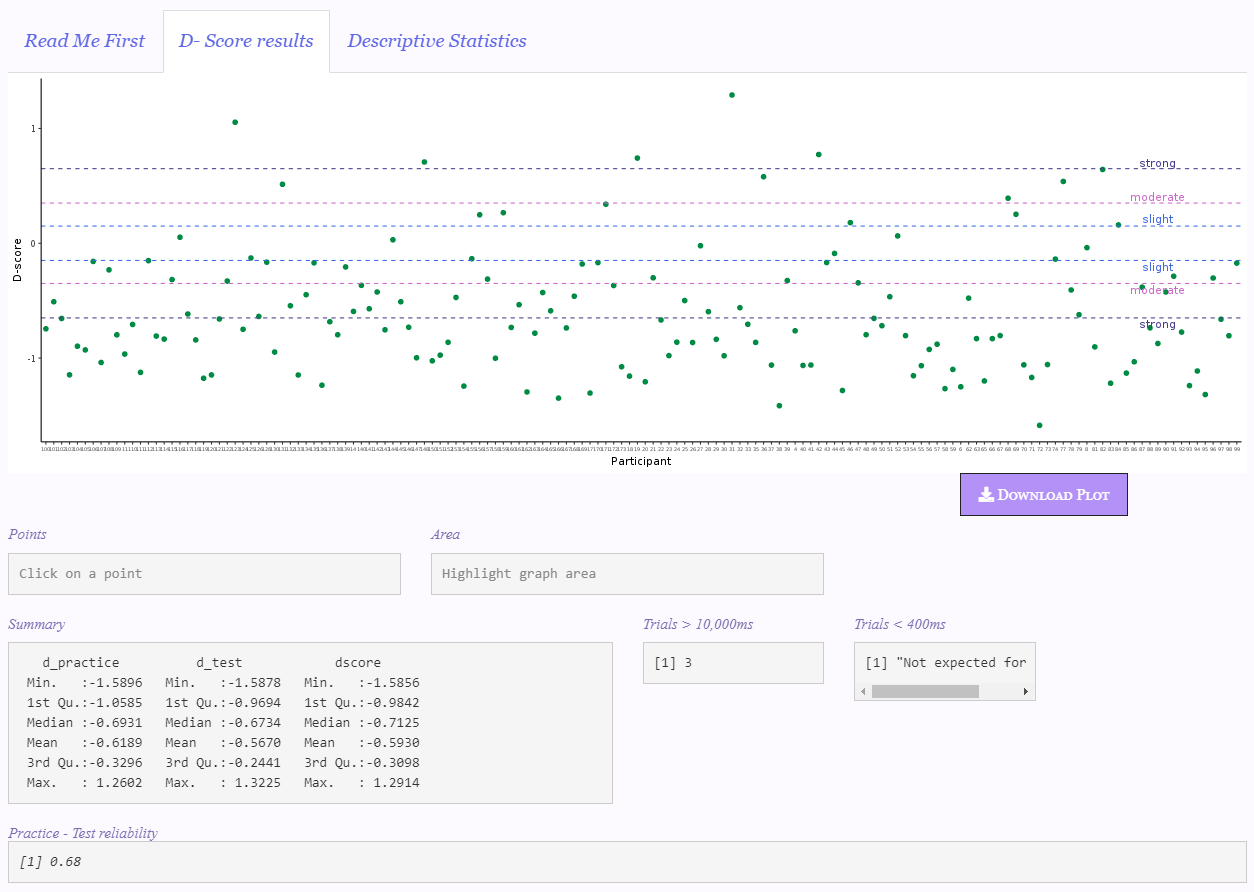
\includegraphics[width=0.8\textwidth]{resultsApp.png}
	\caption{DscoreApp results panel.}
	\label{fig:dscoreapp}
\end{figure}
%
Both descriptive statistics of the results and their graphical representation are available at the same time, and they change interactively as users change the configuration in the ``Input'' panel. 
The \texttt{Summary} box reports the descriptive statistics of the $D_{\text{practice}}$, $D_{\text{test}}$, and the actual \emph{D} score. 
The \texttt{Trials > 10,000ms} box reports the number of trials discarded because of a slow latency (if any), while the \texttt{Trials < 400ms} box reports the number of trials discarded because of fast response times. This box is populated only when a \emph{D} score with fast trials deletion is selected, otherwise the ``Not expected for this D'' label is displayed. 
The \texttt{Practice-Test reliability} box contains the IAT reliability computed as the correlation between associative practice and associative test blocks across participants \cite{gaw2017}.

Graphical representation is a convenient way to identify extreme scores or particular response patterns. Since it might be difficult to link a particular point (or points area) in the graph with the corresponding participants' IDs in the data set, DscoreApp comes with two handy tools designed to access the respondents' IDs from the graph. By clicking on a point in the graph, the ID of the participant that corresponds to the selected point, and his/her \emph{D} score, appears in the \texttt{Points} box. By highlighting an area of the graph, the IDs of participants included in the area, along with their \emph{D} scores appears in  the \texttt{Area} box.
The \texttt{Points} box and the \emph{Area} box are represented in Figure \ref{fig:dscoreapp}, right underneath the graphical representation of the results.

DscoreApp provides users with different options for the graphical representation of the results (Figure \ref{fig:dscoregraph}), at both individual (Figure \ref{fig:point}) and sample (Figure \ref{fig:hist}, \ref{fig:dens}, \ref{fig:histdens}) levels. 
%
\begin{figure}[h!]
	\centering 
	\begin{subfigure}{0.4\linewidth}
		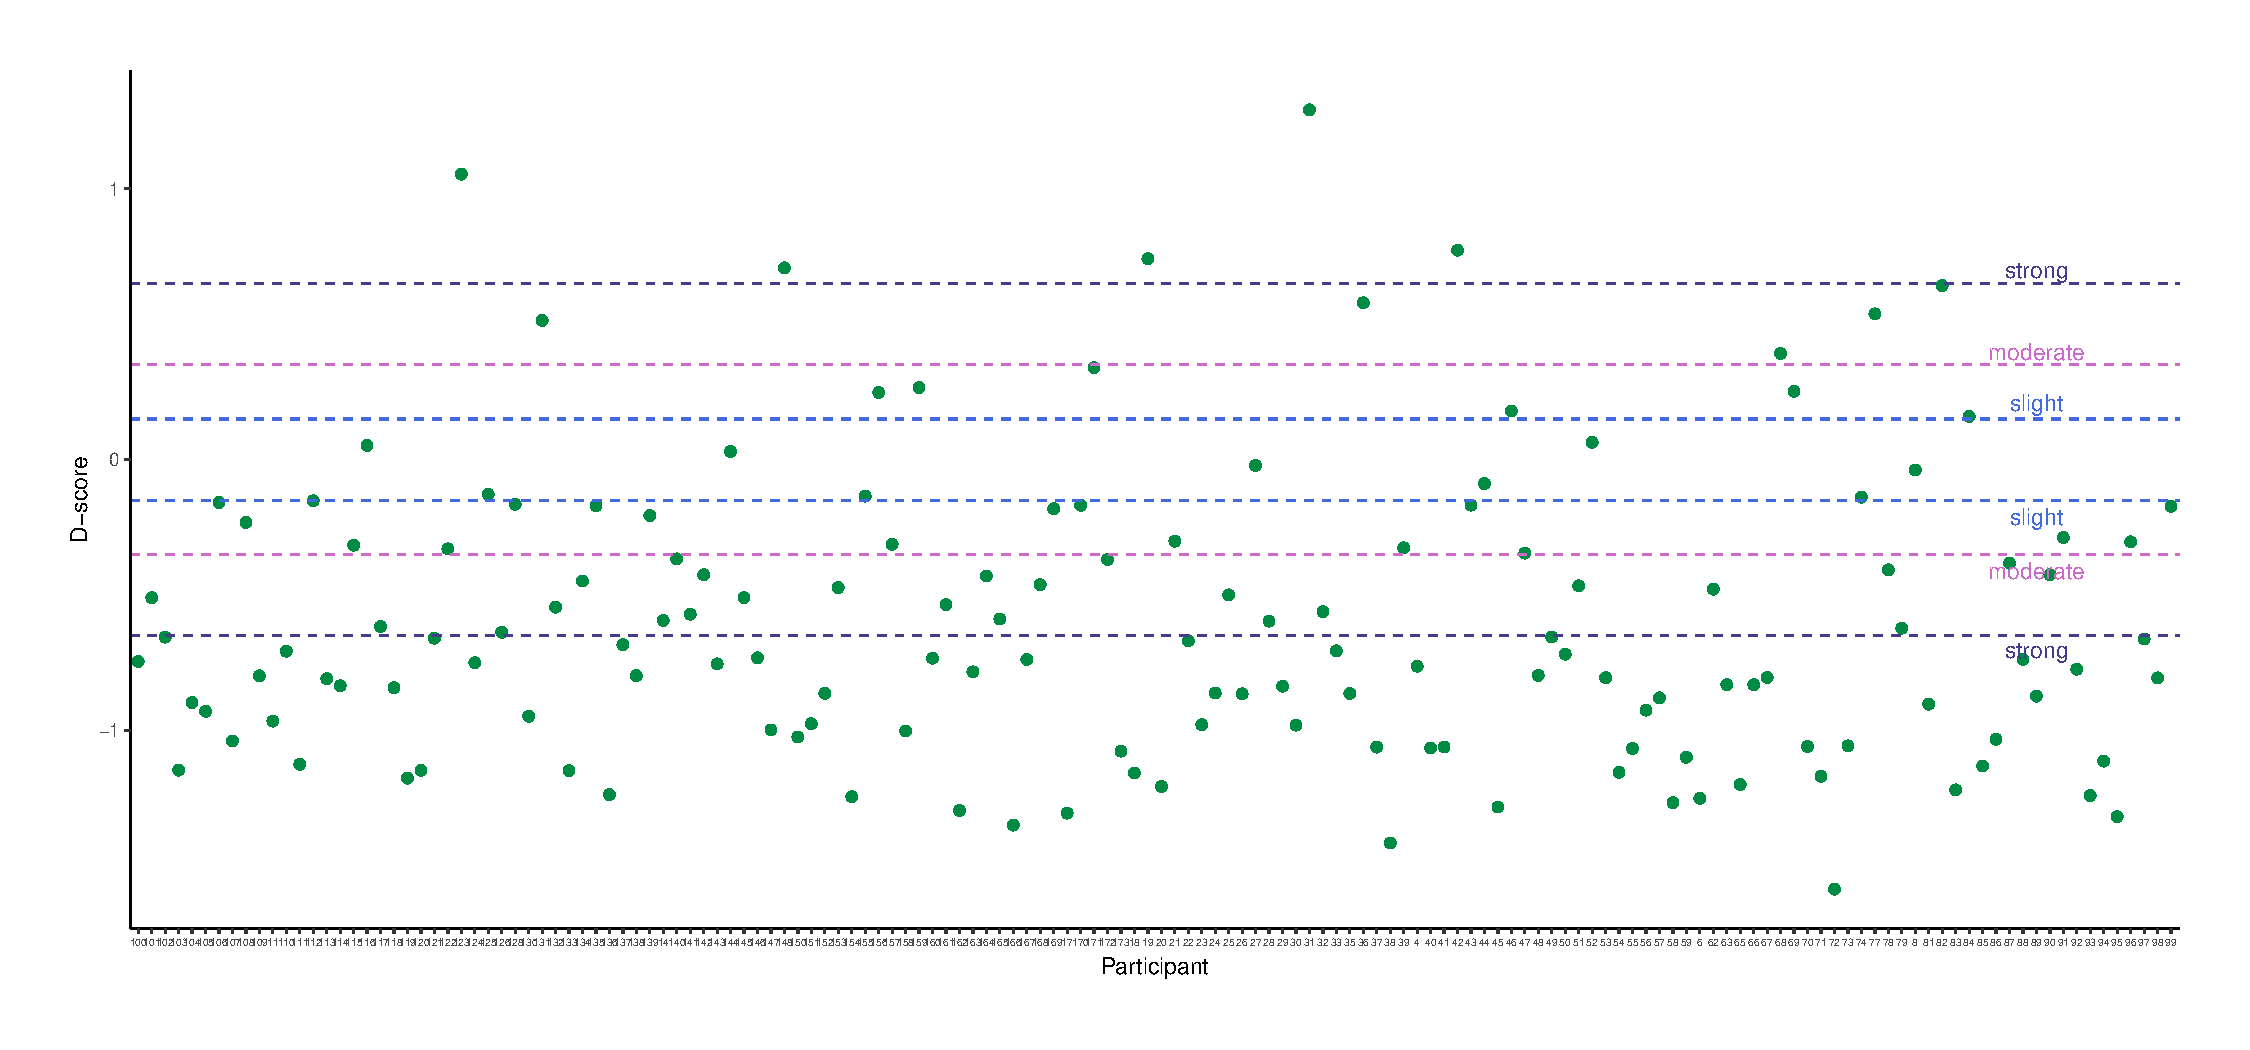
\includegraphics[width=\linewidth]{PointDefaultDscore3.pdf}
		\caption{Points graph.}
		\label{fig:point}
	\end{subfigure}
	\begin{subfigure}{0.4\linewidth}
		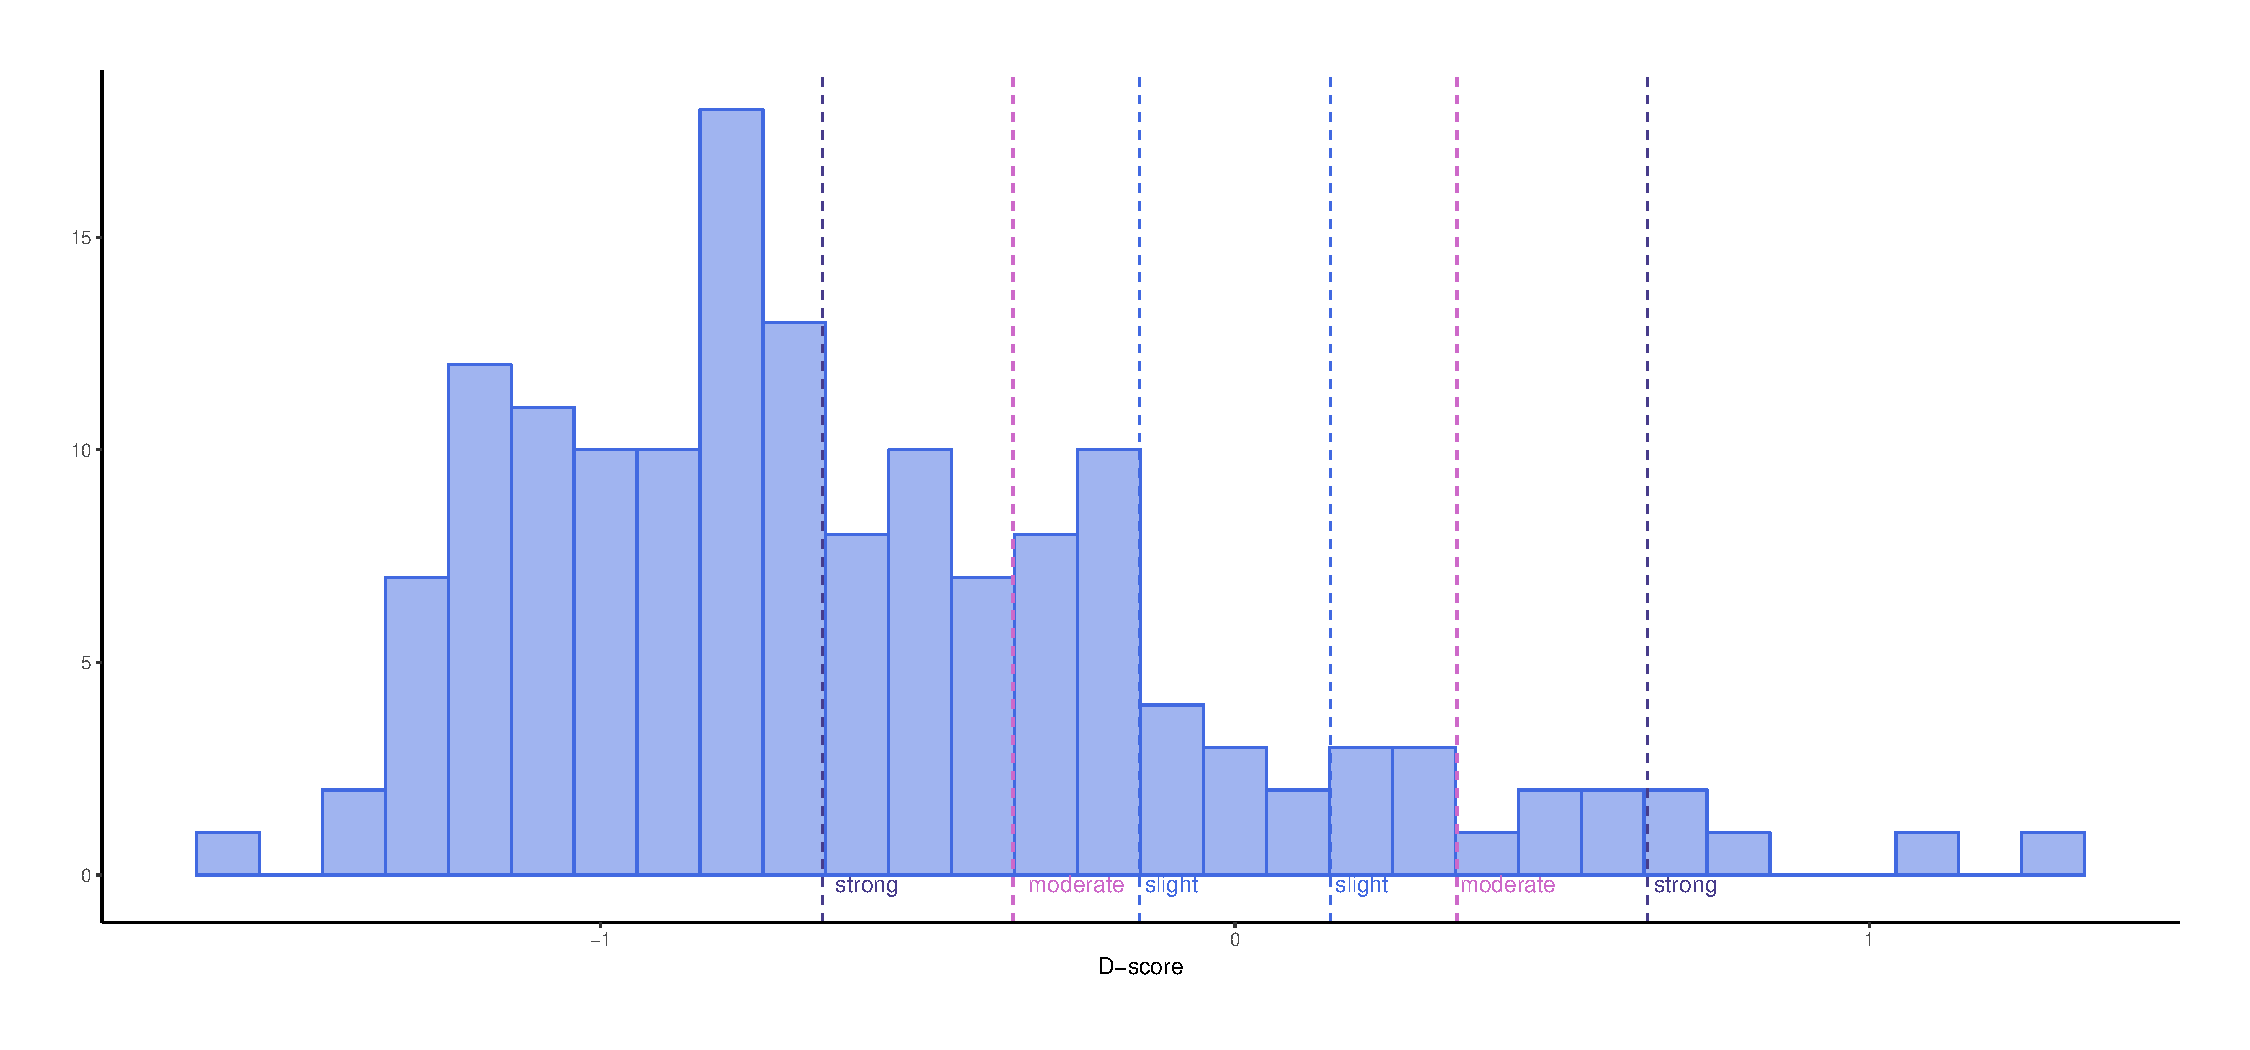
\includegraphics[width=\linewidth]{HistogramDscore3.pdf}
		\caption{Histogram.}
		\label{fig:hist}
	\end{subfigure}
	\begin{subfigure}{0.4\linewidth}
		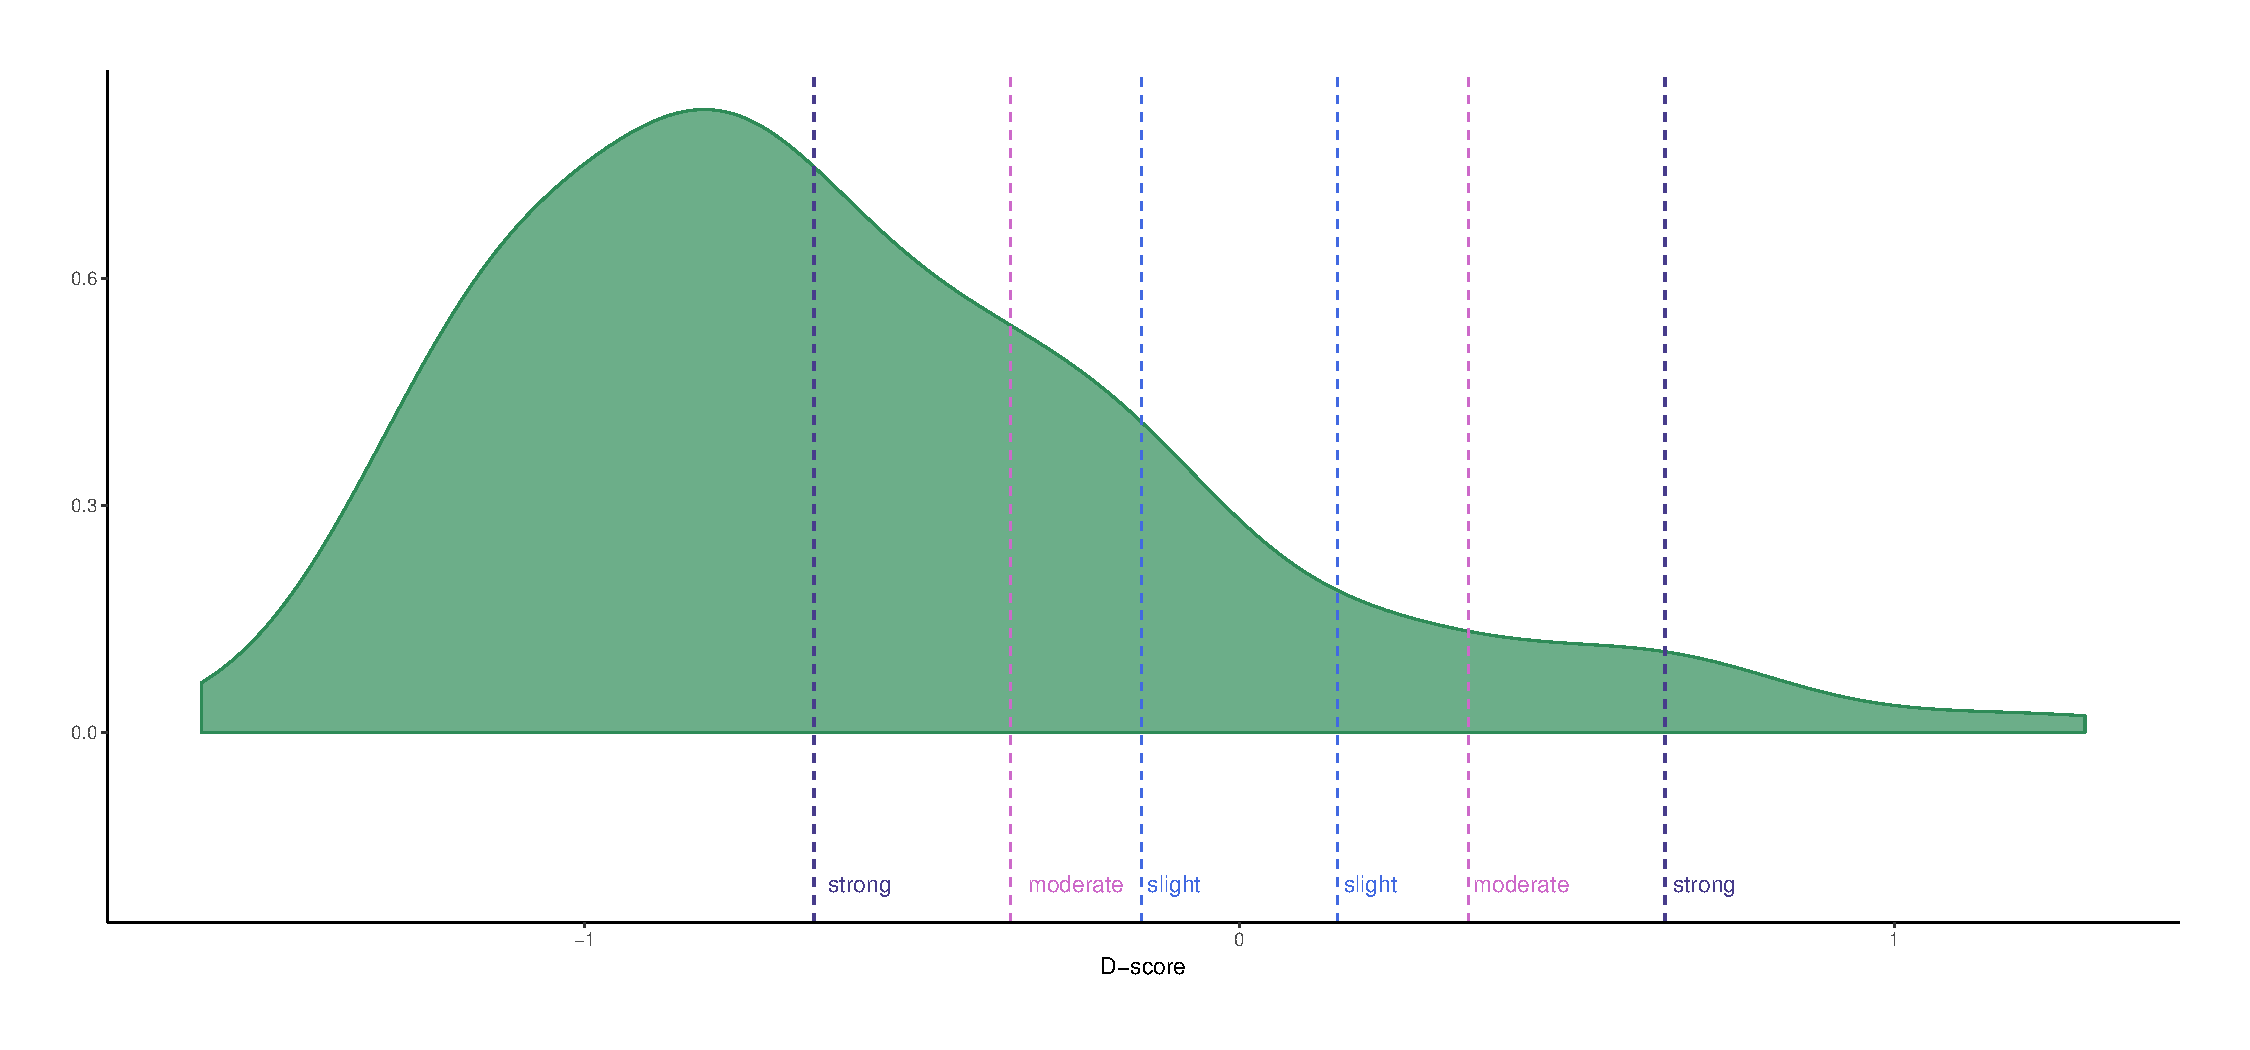
\includegraphics[width=\linewidth]{DensityDscore3.pdf}
		\caption{Density.}
		\label{fig:dens}
	\end{subfigure}
	\begin{subfigure}{0.4\linewidth}
		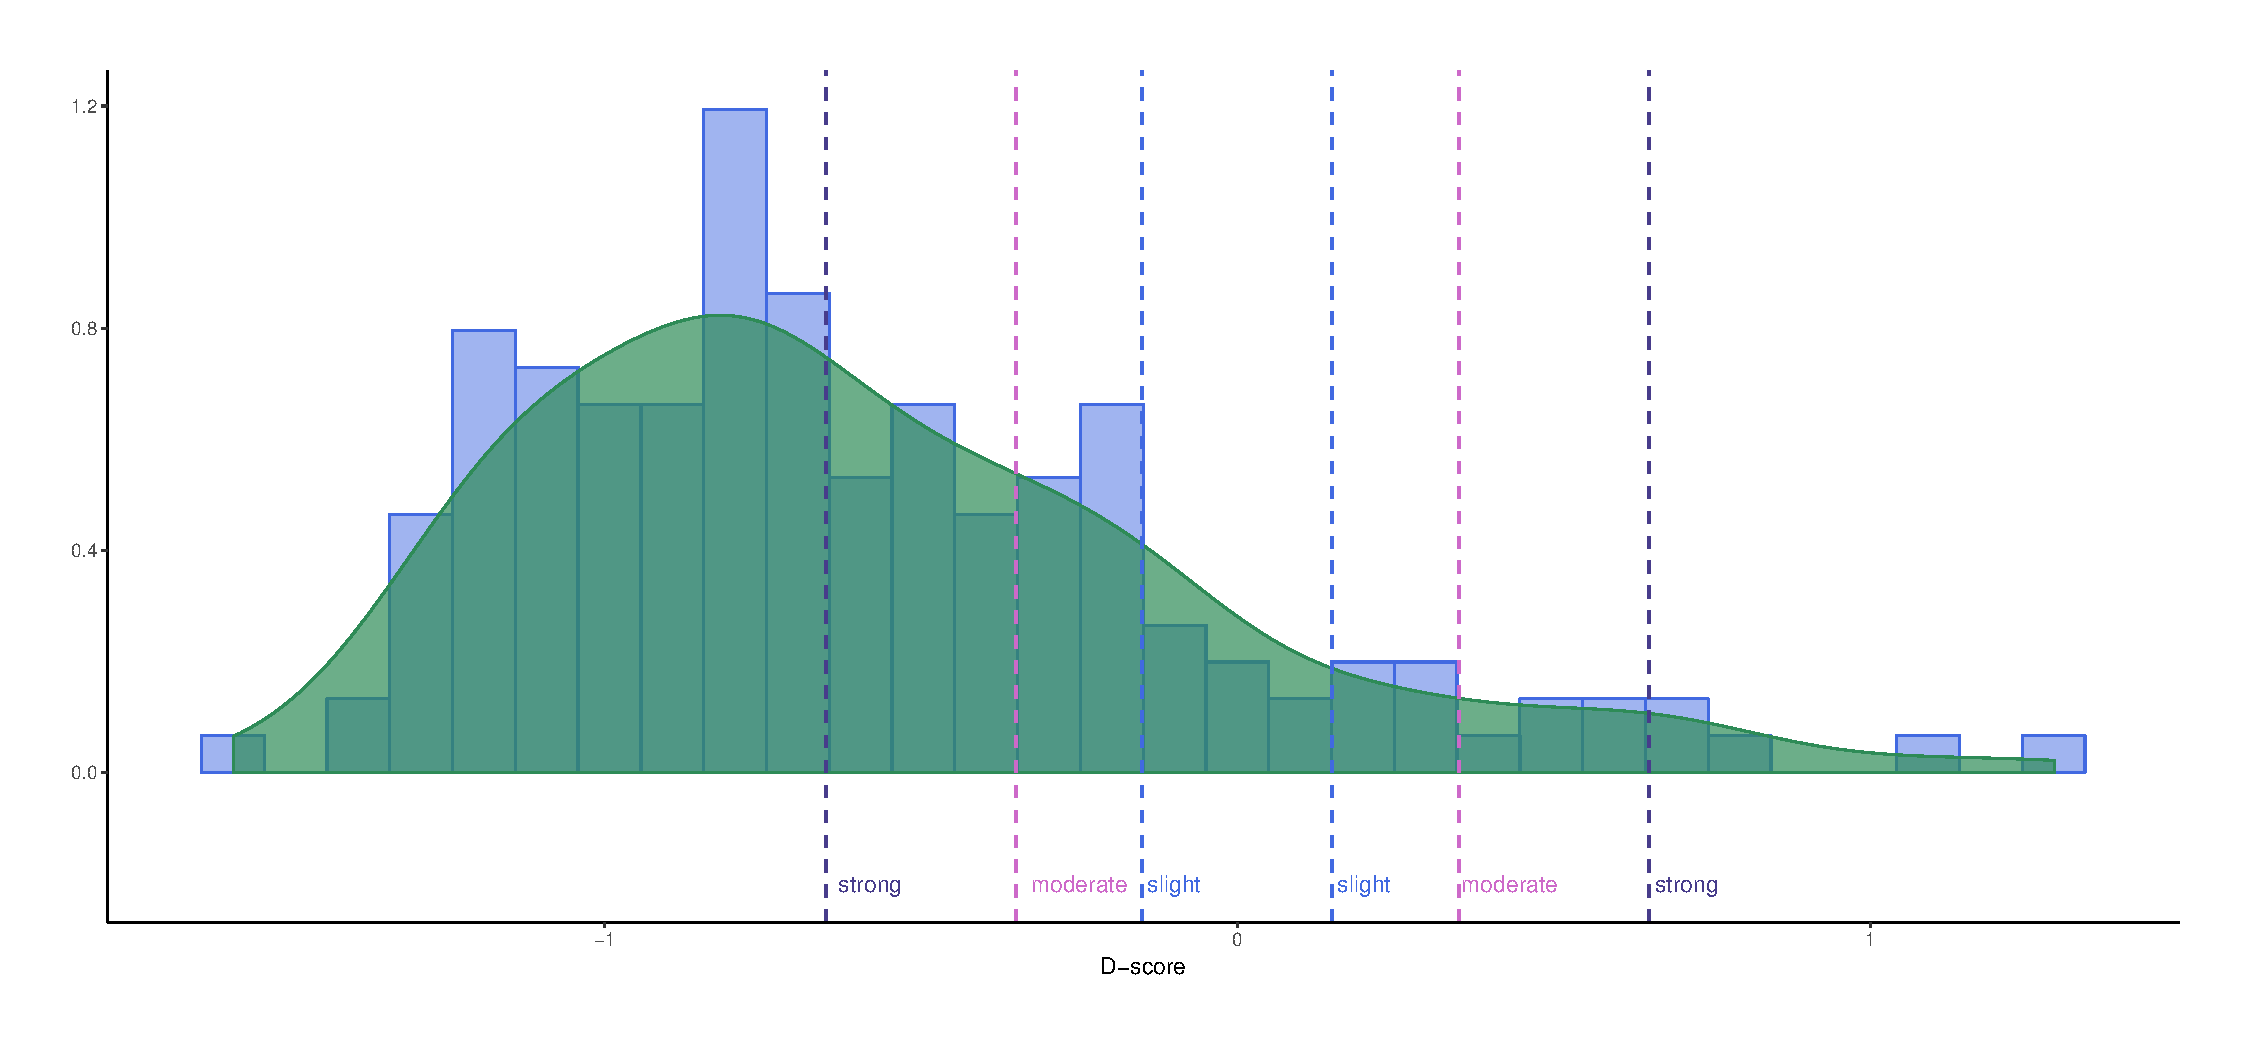
\includegraphics[width=\linewidth]{HistDensDscore3.pdf}
		\caption{Histogram and Density.}
		\label{fig:histdens}
	\end{subfigure}
	\caption{\label{fig:dscoregraph} Available graph representations.}
\end{figure}


All the graphical representations are downloadable in a .pdf format.

\subsection{\texttt{implicitMeasures}}\label{sub:package}

Despite both the IAT and the SC-IAT are commonly used for the implicit assessment of several constructs, \texttt{R} packages for the computation of only the IAT \emph{D} score are available, while there are no packages for computing the SC-IAT \emph{D} score.

Besides the above-mentioned shortcomings of \verb*|R| packages for computing the IAT \emph{D} score, there are also issues related to the replicability of the results.
Researchers' choice on which IAT \emph{D} score algorithm to compute might influence the results and the conclusions that are drawn from them \cite{ellithorpe2015}. Moreover, in many cases researchers fail to report of the exact \emph{D} score algorithm they decided to use \cite{ellithorpe2015}. 
Replicability issues might also rise from mistakes that might be caused by the many steps needed to clean and prepare the starting data set for computing the \emph{D} score \cite{ellithorpe2015}. 

Despite DscoreApp addresses the majority of the replicability issues, it presents some drawbacks as well. Firstly, since the code is into the shiny interface, it cannot be called from the command line, making  impossible to replicate it and hence the results. To be fair, this is a general and outstanding issue concerning shiny apps in general. 
This might not be a concern for general users, but it is indeed a problem in an open science framework where every code should be accessible and replicable with no effort and at any time.
Moreover, the downloadable graphical representations are provided in a pdf format, and hence they cannot be further modified.

The \verb*|implicitMeasures| package \cite{implicit, implicitMeasures} was aimed at addressing the issues concerning both \verb*|R| packages and DscoreApp. It provides an easy and open source way to clean and score both the IAT and the SC-IAT, to easily compare different IAT \emph{D} score algorithms, and to provide clear and customizable plots. Plot functions are all based on \verb*|ggplot2| \cite{ggplot2}. The \verb*|implicitMeasures| package has been published in \citeA{implicitMeasures}.


The source code of \verb*|implicitMeasures| is available on GitHub \\ (\url{https://github.com/OttaviaE/implicitMeasures}). The package is downloadable from CRAN \\ (\url{https://cran.r-project.org/web/packages/implicitMeasures/index.html}).

Table \ref{tab:implicitmeasures} provides an overview of the functions included in the \verb*|implicitMeasures| package.
%
\begin{table}[h!]
	\centering \onehalfspacing
	\caption{\label{tab:implicitmeasures} Contents and functions \texttt{implicitMeasures}.}
	\begin{tabular}{p{5cm} p{9cm}}
		\hline
		Function & Description \\
		\hline

\verb*|clean_iat()|& Prepare and clean IAT data\\
\verb*|clean_sciat()|& Prepare and clean SCIAT data\\
\verb*|compute_iat()|& Compute IAT \emph{D} score \\
\verb*|compute_sciat()|& Compute SCIAT \emph{D} score \\
\verb*|descript_d()|& Print descriptive table of \emph{D} scores (also in \LaTeX) \\
\verb*|d_density()|& Plot either IAT or SCIAT scores (distribution) \\
\verb*|d_point()|& Plot either IAT or SCIAT scores (points) \\
\verb*|IAT_rel()|& Compute IAT reliability \\
\verb*|multi_dsciat()|& Plot scores resulting from two SCIATs\\
\verb*|multi_dscore()|& Compute and plot multple IAT \emph{D} scores\\
\verb*|raw_data()|& Example data set \\
\bottomrule
	\end{tabular}
\end{table}

The \verb*|implicitMeaures| package provides an easy way to compute the algorithms for the both the IAT and the SC-IAT in an automated way. By explicitly referring to the \emph{D} score algorithm that has been used for computing the IAT score in the package, other users can easily replicate the results. 
Additionally, the possibility to compute all available algorithms for the IAT \emph{D} score allows for an easy comparison between them. This makes possible to investigate whether or how the elimination of fast responses or the error replacement strategies affect the results. 

%Indeed, preventing computational mistakes, having a clear reference on the specific \emph{D} score that has been computed, and comparing alternative \emph{D} score algorithms can have a positive influence on the replicability of the results \citeA{ellithorpe2015}.

All objects created with the functions in \verb*|implicitMeasures| functions can be exported in external files. For example, the data frame obtained from the \verb*|clean_iat()| function can be easily exported in a CSV file and then uploaded to DscoreApp (see Section \ref{sec:dscoreapp}).  

The functions for plotting the results are based on \verb*|ggplot2| \cite{ggplot2}, and they can be further modified by users, for instance by taking out the legend, adjusting the figure margins, changing labels and font. All the plots are then exportable as images (.jpg or .png) or as a .pdf.



%\bibliographystyle{apacite} 
%\bibliography{biblioTesi}
\end{document}